\documentclass[withindex, glossary]{cam-thesis}
\pdfminorversion=7

\usepackage[spanish]{babel}
\usepackage[utf8]{inputenc}
\usepackage[T1]{fontenc}
\usepackage[table]{xcolor}
\usepackage{multirow}
\usepackage{tabularx}
\usepackage{graphicx}
\usepackage{lmodern}
\usepackage{cleveref}
\usepackage{amsmath}

\usepackage{hyperref}
\addto\extrasspanish{%
    \def\chapterautorefname{capítulo}%
}

\usepackage{svg}
\usepackage{multicol}
\usepackage{mathtools}
\usepackage{booktabs}
\usepackage{bookmark}
\usepackage{blkarray, bigstrut}
\usepackage{subcaption}
\usepackage{pgfgantt}
\usepackage{array}
\usepackage[capposition=top]{floatrow}

\usepackage[backend=biber, style=ieee, sorting=ynt]{biblatex}
\addbibresource{thesis.bib}

\usepackage{minted}
\usemintedstyle{manni}

\usepackage{csquotes}

\usepackage{tikz}
\usetikzlibrary{shapes.geometric, arrows.meta, fit, backgrounds, positioning, matrix, decorations.pathreplacing, calc}
\tikzstyle{startstop} = [rectangle, rounded corners, minimum width=3cm, minimum height=1cm,text centered, draw=black, fill=red!50]
\tikzstyle{io} = [trapezium, trapezium left angle=70, trapezium right angle=110, minimum width=3cm, minimum height=1cm, text centered, draw=black, fill=blue!30]
\tikzstyle{process} = [rectangle, minimum width=3cm, minimum height=1cm, text centered, draw=black, fill=orange!30]
\tikzstyle{decision} = [diamond, minimum width=3cm, minimum height=1cm, text centered, draw=black, fill=green!20]
\tikzstyle{database} = [cylinder, minimum width=3cm, minimum height=2cm, text centered, shape border rotate=90, aspect=0.25, draw=black, fill=yellow!30]
\tikzstyle{arrow} = [thick, ->, >=stealth]
\tikzstyle{line} = [-Latex]
\newcommand{\inline}[2]{%
    \begin{tikzpicture}[baseline=(word.base), txt/.style={shape=rectangle, inner sep=0pt}]
        \node[txt] (word) {\texttt{#1}};
        \node[above] at (word.north) {\footnotesize{#2}};
    \end{tikzpicture}%
}

\usepackage{pgfplots}
\pgfplotsset{compat=newest}

\setlength{\columnseprule}{0.4pt}
\linespread{1.25}


\title{Máster Universitario en Computación Gráfica y Simulación\protect\\\bigskip \normalfont{2018\protect\\\bigskip Trabajo Final de Máster\protect\\\bigskip Estudio sobre sistemas de anti-aliasing e implementación de anti-aliasing temporal}}
\author{Hugo Ferrando Seage}
\submissiondate{Tutor: Dr.~Alberto Sánchez Campos}

% PDF meta-info
\subjectline{Máster en Computación Gráfica y Simulación}
% max 6
\keywords{opengl anti-aliasing temporal}

% Abstract
\espabstract{%
    Debido a la resolución limitada de las pantallas al \gls{rasterizar} gráficos 3D se deforman ciertas lineas y curvas. Este fenómeno se llama aliasing. La demanda de gráficos cada vez más realistas ha propiciado la creación de diferentes técnicas y algoritmos para disimular estos defectos, sin tener que recurrir necesariemente a pantallas de mayor resolución.

    El anti-aliasing se ha vuelto una técnica crucial para mejorar la calidad de imagen en el software con gráficos tridimensionales. Este campo de la computación gráfica lleva años desarrollandose, con nuevas técnicas publicadas continuamente.

    Este proyecto tiene como objetivo el análisis de las distintas técnicas existentes en el estado del arte y la implementación de un algoritmo de anti-aliasing temporal, compatible con motores con deferred shading y comparable en calidad al multisampling, junto a otras propiedades.
}

\abstract{%
    When rasterizing 3D graphics using computer screens, due to their limited resolution, some lines and curves will become deformed. This phenomena is called aliasing. The ever increasing demand for more realistic graphics has driven the creation of new techniques and algorithms to hide these artifacts, without necessarily using higher resolution screens.

    Anti-aliasing has become a crucial technique to advance image quality in graphics software. This field has been explored for years, with new approaches being developed continually.

    This projects aims to analyze different anti-aliasing techniques developed and the implementation of a temporal anti-aliasing technique, compatible with deferred shading engines and with a similar quality to multisampling, amongst other benefits.
}

% Glossary
\newglossaryentry{rasterizar}{%
    name=rasterizar,
    description={Conversión de una imagen descrita con alguna primitiva (curvas, vectores, triangulos) a un conjunto de pixels}
}

\newglossaryentry{opengl}{%
    name=OpenGL,
    description={API estándar para el desarollo de software con gráficos 2D o 3D con aceleración por hardware\cite{Kessenich:2016:OPG:3013620}}
}

\newglossaryentry{DSLR}{%
    name=DSLR,
    description={Digital single-lens reflex camera. Cámara fotográfica digital con una única lente y sensor electrónico}
}

\newglossaryentry{FPS}{%
    name=FPS,
    description={Frames per second. Número de fotogramas por segundo. En software gráfico refleja el rendimiento del mismo}
}

\newglossaryentry{SSAO}{%
    name=SSAO,
    description={Screen Space Ambient Occlusión. Técnica gráfica para calcular la exposición a la luz ambiente en cada punto de una escena}
}

\newglossaryentry{TXAA}{%
    name=TXAA,
    description={Anti aliasing temporal desarrollado por Nvidia}
}

% Acronyms

% Contents
\begin{document}
\frontmatter{}

% Thesis body:
\chapter{Introducción}

La calidad de imagen exigida en las aplicaciones gráfica es cada vez mayor, tanto en ámbitos lúdicos como para la generación de efectos visuales en películas o en videojuegos, como en aplicaciones civiles, educativas, médicas\cite{rayos}, o psicológicas. El realismo exigido por los usuarios es grande, pues el entrenamiento permanente de consumo de gráficos por ordenador ha provocado que las expectativas de cualquier gráfico o imagen sean elevadas. Si bien la tecnología no ha parado de avanzar, la calidad exigida tanto en aplicaciones 2D como 3D provoca la eminente necesidad de optimizar procesos de simulación o renderizado.

Una de las técnicas a optimizar es el anti-aliasing, ya que aporta más credibilidad a cualquier escena 3D e incluso en imágenes 2D. Uno de los ámbitos donde es imprescindible el anti-aliasing es en el renderizado de textos de los sistemas operativos gráficos, como los de escritorio o móviles. Los programas de edición de imágenes también cuentan con numerosos algoritmos de anti-aliasing con el objetivo de mejorar las imágenes o fotos.

Debido a la resolución limitada de las pantallas, será necesario usar este tipo de técnicas para emular la calidad que ofrecen las pantallas con una mayor densidad de pixels. Por la potencia del hardware actual, las técnicas tradicionales como el supersampling para realizar dicho efecto es impráctico. Por esa razón ha sido necesario el desarrollo de algoritmos más sofisticados que alcanzan una calidad similar, pero con un impacto en el rendimiento más asequible.

En definitiva, el aliasing es un problema fundamental en la computación gráfica y a día de hoy no existen ningún algoritmo perfecto que lo solucione a tiempo real. Por ese motivo existen una multitud de alternativas, cada una con sus ventajas e inconvenientes, que se exploran en este trabajo final de máster.

\chapter{Planteamiento del problema}

El aliasing siempre ha sido un problema en el campo de la computación gráfica. Desde la década de los 70 se han usado técnicas como la interpolación bicubica para el renderizado de imágenes por ordenador con ray-tracing.

Durante la década de los 80 y buena parte de los 90 hubo un avance constante en términos de potencia, resolución y la capacidad de mostrar cada vez más colores (por ejemplo del paso de gráficos CGA a VGA). Aún así el rendimiento necesario para aplicar muchas de las técnicas de anti-aliasing solo se podían usar con workstations profesionales, como las IRIS de Silicon Graphics.

A mediados de los 90, con la llegada de la tarjetas aceleradores de gráficos 3D a ordenadores más modestos, las compañías como ATI, NVIDIA y 3DFX empezaron a integrar soluciones de anti-aliasing a sus productos y APIs.

A la vez que evolucionaba el hardware los gráficos cada vez requerían más potencia. Las técnicas como el supersampling reducen drásticamente el rendimiento, por lo que en muchos casos se empezaron a usar optimizaciones como el multisampling.

Con la llegada de los shaders programables y el deferred shading el multisampling empezó a no poder ser usado en muchos casos. Por ello se desarrollaron algoritmos como el MLAA, FXAA y SMAA que son compatibles tanto con el forward shading como el deferred shading y con un impacto muy bajo en el rendimiento.

Al contrario que el supersampling, el multisampling y el post-processing anti-aliasing no solucionan todos los tipos de aliasing que tiene una imagen. Para intentar aunar las ventajas del supersampling con el rendimiento y compatibilidad del post-processing anti-aliasing se han empezado a desarrollar técnicas de anti-aliasing temporal, como el \GLS{TXAA}\@.

\chapter{Objetivos}

Este proyecto tiene dos objetivos principales:

\begin{enumerate}
    \item Analizar el estado del arte en el campo de la computación gráfica en relación al anti-aliasing. Explorar los problemas que presenta el aliasing en gráficos 2D y 3D, la evolución de las soluciones y los desarrollos en curso.
    \item El segundo objetivo es el de integrar una solución de anti-aliasing temporal para mejorar la calidad de imagen de un motor gráfico. El resultado final deberá tener una calidad equivalente a la de otras soluciones más convencionales como el supersampling, pero con un impacto en el rendimiento mucho menor, como con un post processing aliasing tradicional (FXAA, SMAA).
\end{enumerate}

\chapter{Estado del Arte}

\section{Tipos de Aliasing}

El aliasing es la deformación de ciertos elementos gráficos al ser rasterizados y plasmados en una pantalla con una resolución finita\cite{Mitchell:1988:RFC:378456.378514}. Normalmente los bordes de la geometría que tengan ángulos que no se alineen perfectamente con los pixels presentarán bordes de sierra abruptos, que no son fieles a la escena como se vería de forma natural.

Este proyecto se centra en aliasing dentro del campo de la computación gráfica, pero afecta a otras disciplinas, como el procesamiento de señales (por ejemplo al digitalizar señales de audio analógicas). En general, al representar valores continuos en algún medio discreto siempre habrá algún defecto de este tipo\cite{Mitchell:1988:RFC:378456.378514}. Además el aliasing no solo es un problema en aplicaciones lúdicas. En al figura~\ref{skull} se puede apreciar aliasing en una radiografía.

\begin{figure}[!htbp]
    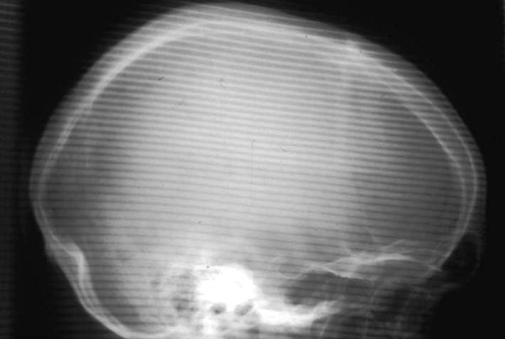
\includegraphics[width=.7\linewidth]{figures/skull.jpg}
    \caption{Aliasing en una radiografía\cite{rayos}}
    \label{skull}
\end{figure}

Existen otros tipos de aliasing, como en el interior de texturas o al mover la camera rápidamente.

\subsection{Aliasing en bordes de geometría}

Seguramente el aliasing más común y conocido en cuanto a la computación gráfica. Es un efecto que se produce en los bordes de la geometría de la escena. Este efecto se manifiesta como un borde con dientes de sierra, como en la figura~\ref{hitmanaliasing}. Es apreciable sobre todo en líneas diagonales y en curvas, ya que en lineas planas (tanto horizontales como verticales) se alinean con el array de pixels de la pantalla.

Esto es debido al point sampling que se emplea durante el rasterizado de la escena (figura~\ref{pointsampling}).

Este tipo de aliasing también está muy ligado a la densidad de la pantalla donde se este viendo la escena. En un display con una densidad de pixels muy alta, siempre que el renderizado sea hecho con la misma resolución que la pantalla, será más difícil apreciar este tipo de aliasing. Aún así, con la tecnología actual, la densidad no siempre es lo suficientemente alta. Por ejemplo, una pantalla UHD (resolución $3840 \times 2160$) de 65'' tiene una densidad de 67.78 DPI, donde el aliasing sigue siendo notable.

En pantallas de alta densidad (> 200 DPI\cite{googledpi}), como la de varios smartphones, este tipo de aliasing no se manifestará.

\begin{figure}[!htbp]
    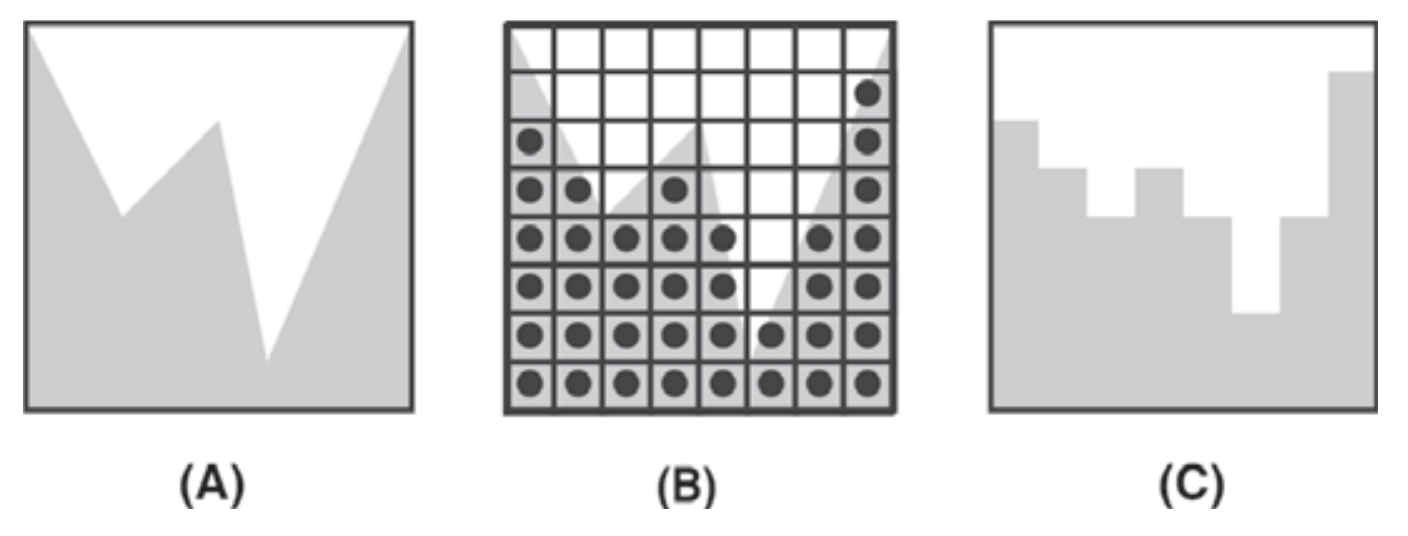
\includegraphics[width=.7\linewidth]{figures/pointsampling.png}
    \caption{Point Sampling\cite{Shreiner:2013:OPG:2544032}}
    \label{pointsampling}
\end{figure}

\begin{figure}[!htbp]
    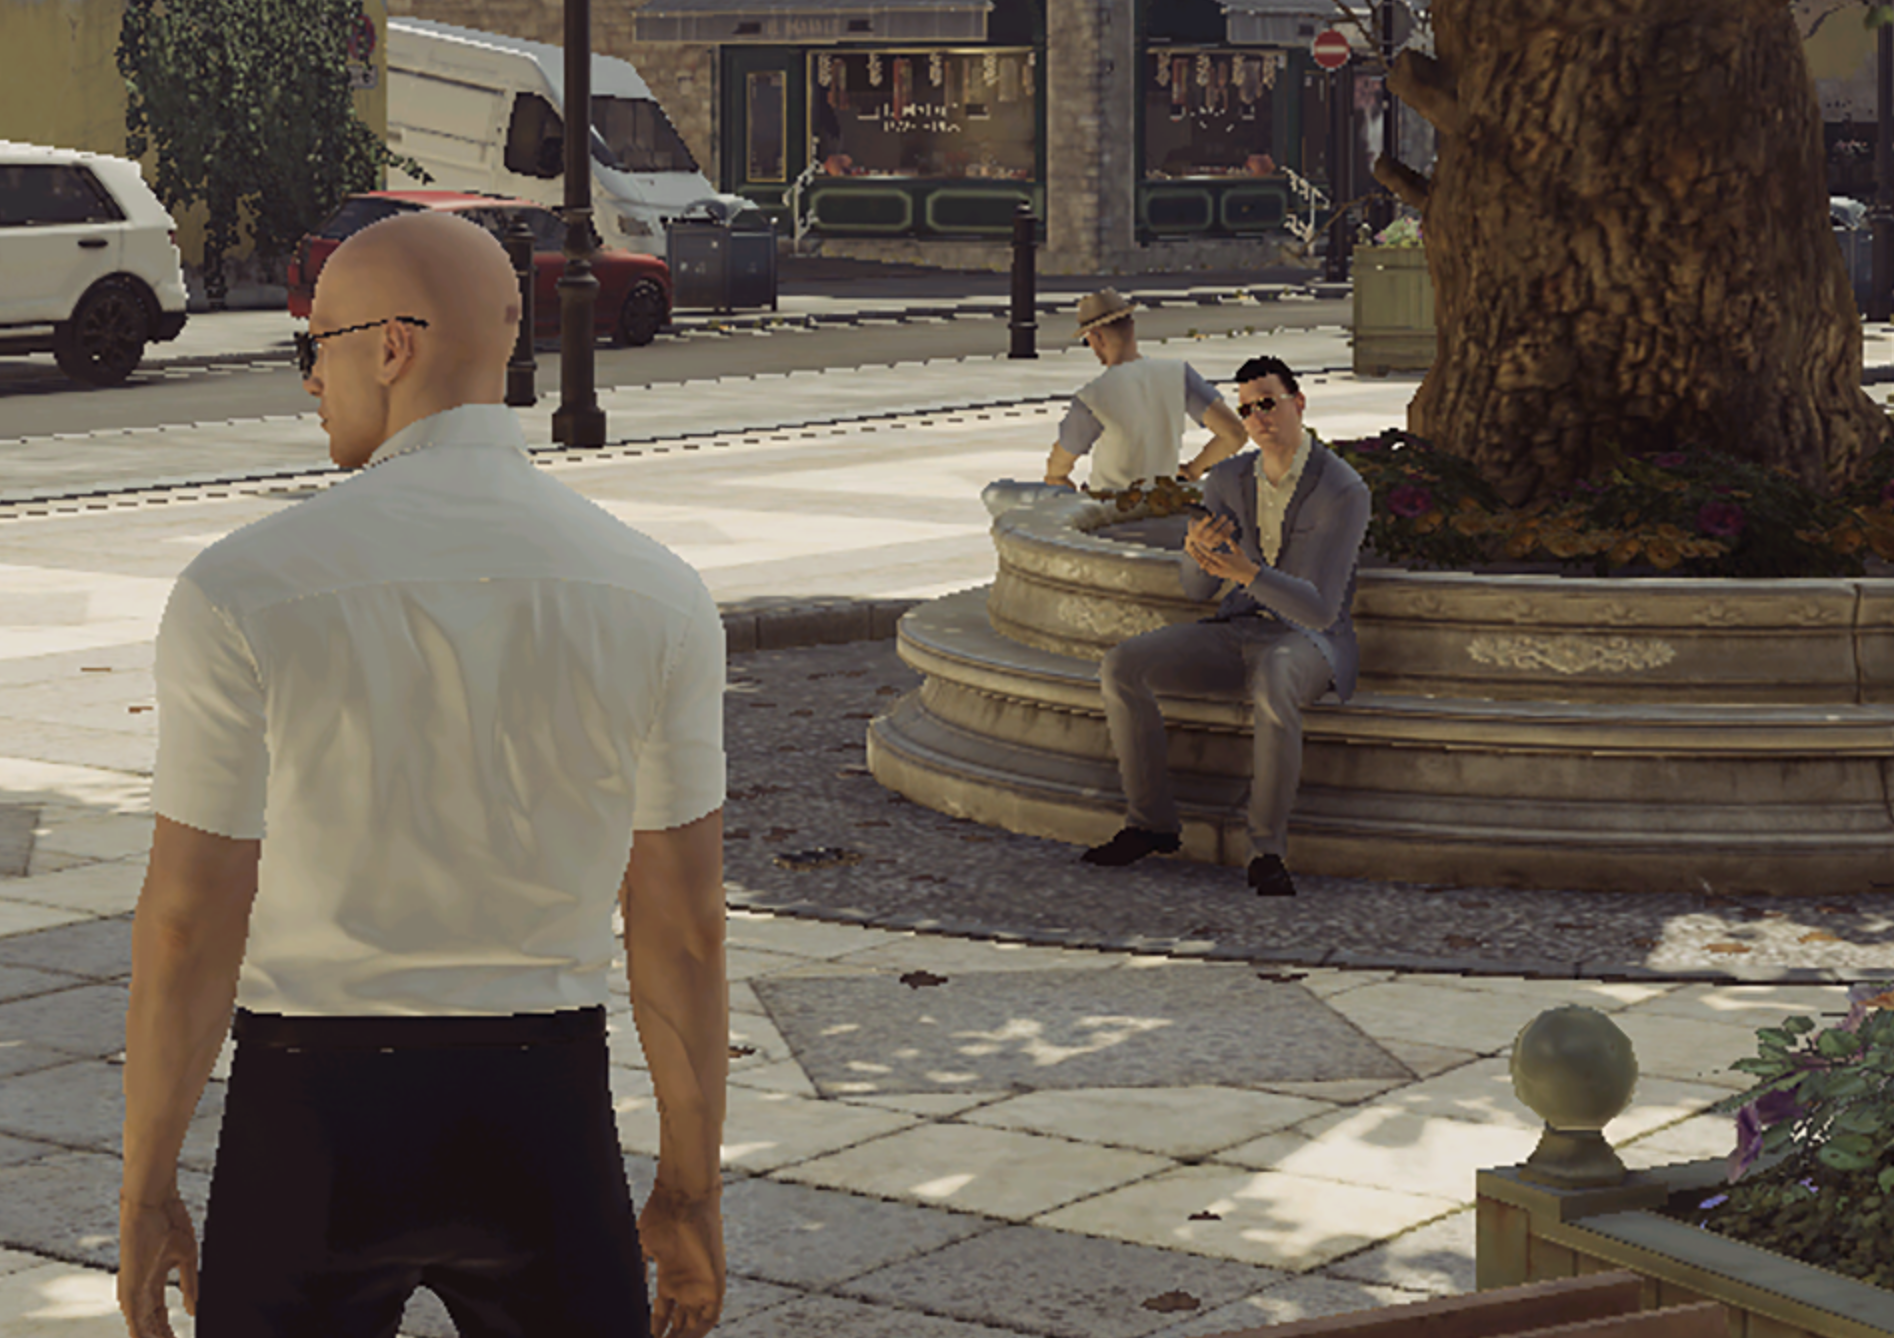
\includegraphics[width=.8\linewidth]{figures/hitmanaliasing.png}
    \caption{Aliasing en Hitman (2016)}
    \label{hitmanaliasing}
\end{figure}

\subsection{Aliasing de texturas}

Dentro de las texturas también puede haber aliasing. Al igual que pasa en los bordes de la geometría, al cambiar de un color a otro rápidamente, debido al sampling limitado, se pueden producir estos mismos defectos.

Este tipo de aliasing no está limitado al rendering de gráficos 3D en tiempo real, si no que se puede apreciar incluso en imágenes con una alta resolución. En estos casos, dependiendo de la textura, se puede ver un patrón de Moiré, como en la figura~\ref{moire}.

\begin{figure}[!htbp]
    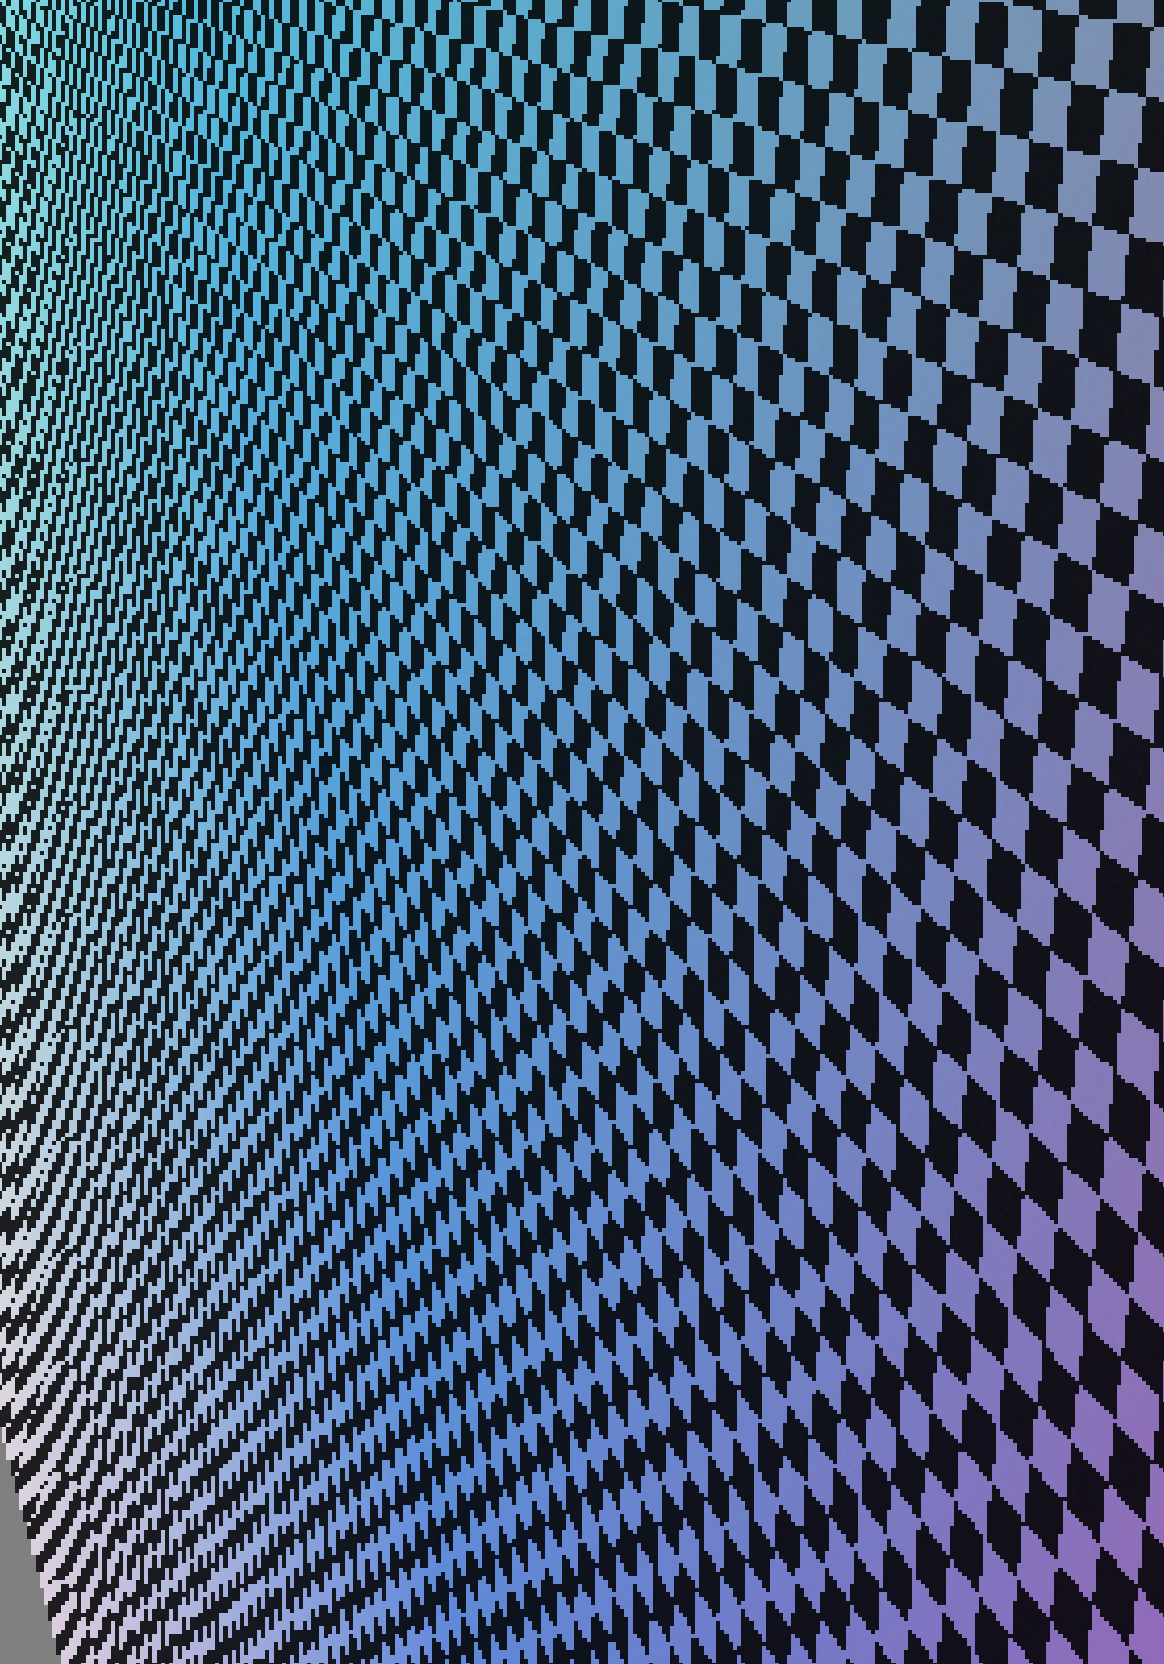
\includegraphics[width=.3\linewidth]{figures/moire.png}
    \caption{Patrón de Moiré\cite{studysupersampling}}
    \label{moire}
\end{figure}

La generación de MIP Maps puede solucionar este tipo de aliasing en ciertas condiciones. Los MIP Maps son versiones alternativas de las texturas usadas por un software gráfico. Estas versiones contienen texturas de menor resolución filtradas, lo que puede aliviar el aliasing y patrones de Moiré producidos por usar downsampling de texturas con una alta resolución con nearest neighbor, como se puede apreciar en la figura~\ref{mipmaps}.

Estas texturas se suelen usar para objetos que estén a alguna distancia determinada de la cámara. Si se pre-filtrasen las texturas originales serían demasiado borrosas y se empeoraría su calidad.

\begin{figure}[!htbp]
    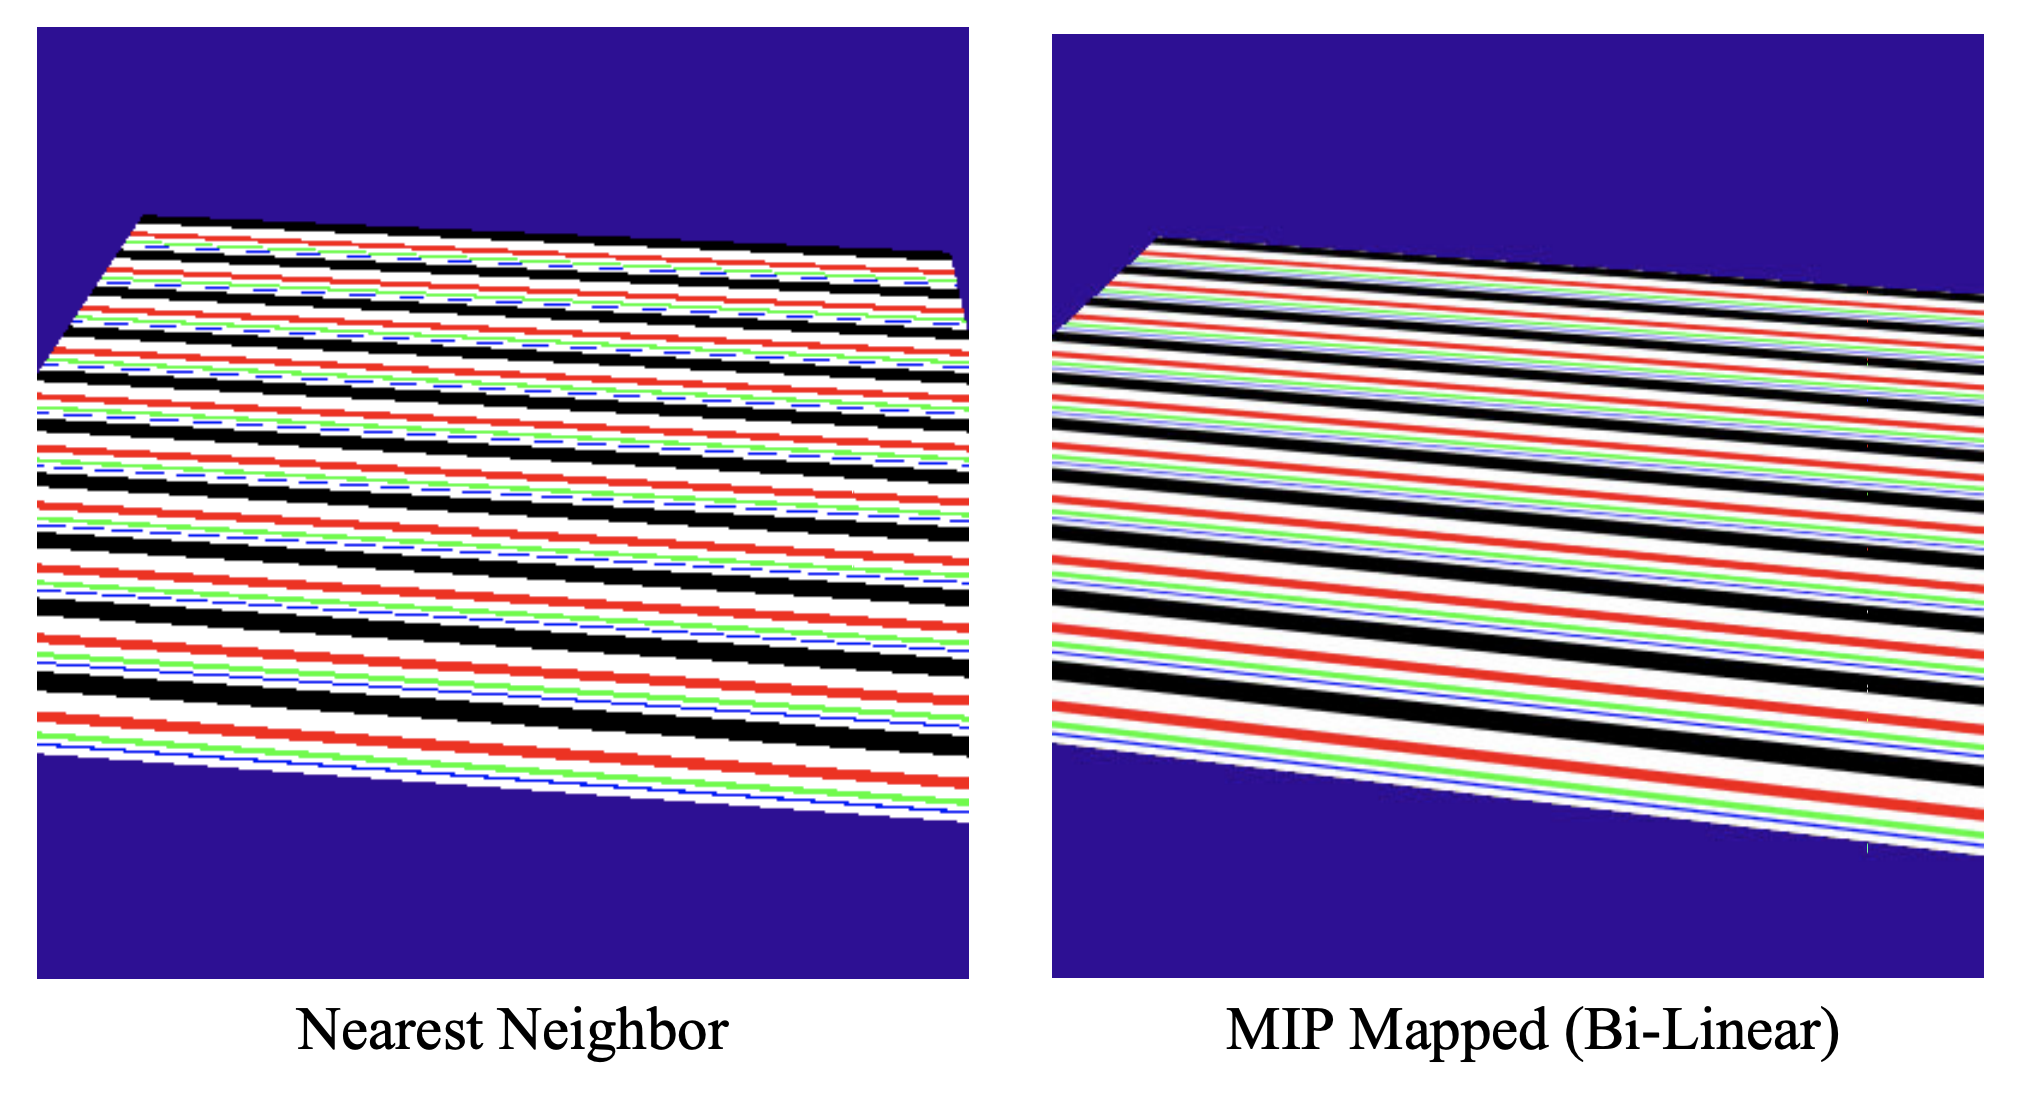
\includegraphics[width=.8\linewidth]{figures/mipmaps.png}
    \caption{Anti-aliasing con Mip Maps}
    \label{mipmaps}
\end{figure}

\subsection{Specular Aliasing}

El modelo clásico de iluminación usado en \Gls{opengl} consiste en componentes de luz ambiente, difusa y especular\cite{Shreiner:2013:OPG:2544032}. La iluminación especular se produce cuando la luz incide directamente sobre un material. Las propiedades del objeto dictarán como de brillante aparece.

Por ejemplo, un espejo es completamente especular, ya que refleja toda la luz que recibe. Otros materiales muy especulares son algunos metales y plásticos. En cambio, la pizarra es un objeto con un valor especular muy bajo y que no producirá apenas reflejos.

\begin{figure}[!htbp]
    \centering
    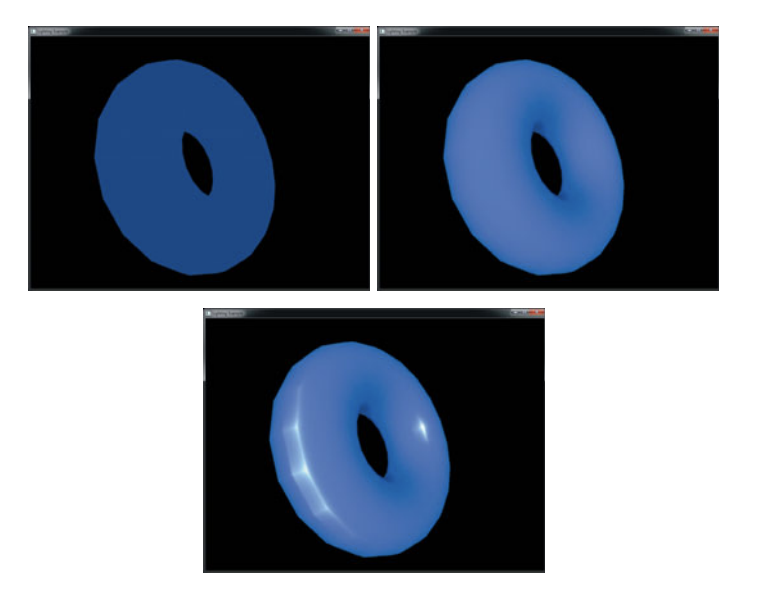
\includegraphics[width=.8\linewidth]{figures/iluminacion.png}
    \caption{Componentes de iluminación en \Gls{opengl}\@. Ambiente (superior izquierda), difuso (superior derecha) y especular (inferior)\cite{Shreiner:2013:OPG:2544032}}
    \label{gls}
\end{figure}

El cálculo de esos reflejos pueden contener aliasing, al igual que las texturas. En la figura~\ref{specular} se puede apreciar como los reflejos de un suelo metálico debido al mismo problema que en el aliasing dentro de texturas.

\begin{figure}[!htbp]
    \centering
    \begin{subfigure}[b]{0.8\textwidth}
        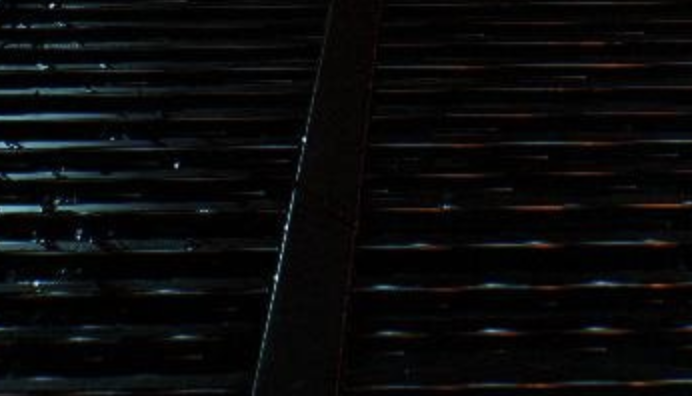
\includegraphics[width=\textwidth]{figures/specular-aliasing.png}
        \caption{Anti-aliasing desactivado}
    \end{subfigure}
    \centering
    \begin{subfigure}[b]{0.8\textwidth}
        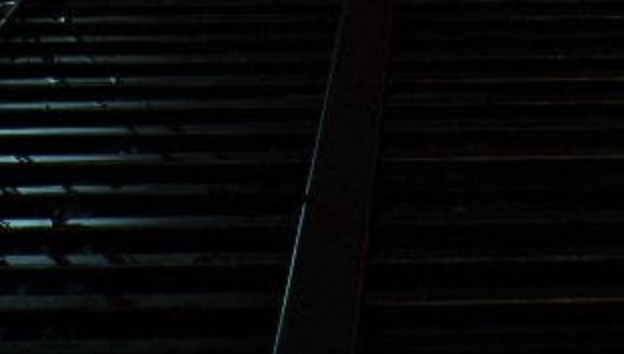
\includegraphics[width=\textwidth]{figures/specular-fixed.png}
        \caption{TSSAA}
    \end{subfigure}
    \caption{Specular aliasing en Doom (2016)}
    \label{specular}
\end{figure}

\subsection{Motion Aliasing}

A veces al mover la cámara también se pueden producir efectos de aliasing. El efecto no se puede apreciar en una imagen fija, pero al verlo el movimiento es un efecto que distrae. Recuerda al parpadeo de una luz, que una vez que la cámara permanece quieta desaparece (también conocido como crawling).

Este tipo de aliasing se suele solucionar con técnicas de blurring, que recuerdan más al efecto del cine a 24\GLS{FPS} que a técnicas de anti-aliasing como las que se explican en los siguientes secciones.

Estos efectos tienen como objetivo simular el efecto que tiene el tiempo de exposición en una cámara. El tiempo de exposición es el tiempo que el objetivo tiene para capturar luz para cada frame de un vídeo, o para una foto. Normalmente, en cine se usa 1/48 de segundo\cite{shuttertips}. Cuanto más tiempo de exposición más blur habrá (aunque los fotogramas serán más claros). En la figura~\ref{shutter} se puede ver el efecto que tienen los diferentes tiempos de exposición en una \GLS{DSLR}\@.

\begin{figure}[!htbp]
    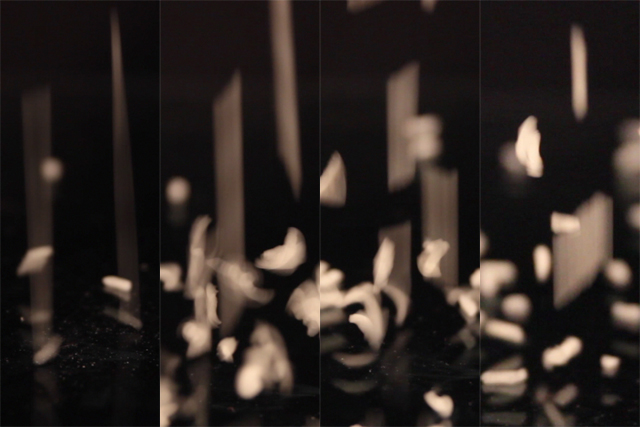
\includegraphics[width=.8\linewidth]{figures/shutter.jpg}
    \caption{Comparación de tiempo de exposición (360º, 180º, 90º, 45º)\cite{shuttertips}}
    \label{shutter}
\end{figure}

Una de las primeras técnicas era la de usar un buffer de acumulación. Consiste en escoger una ventana de $n$ frames anteriores al actual y combinarlo con una opacidad variable. Con cada frame esta ventana se actualiza. Esto intenta emular como funciona el tiempo de exposición de una cámara. Su principal ventaja es que funciona con objetos translucidos y partículas sin tener que hacer nada en especial, ya que afecta a toda la escena. Si el framerate es muy alto (alrededor de 120\GLS{FPS}) y fluido el resultado puede ser muy bueno, pero en software donde el rendimiento es menor (menos de 60\GLS{FPS}) la imagen se verá demasiado borrosa y el efecto no será el deseado. De hecho como se puede ver en la figura~\ref{gta3} puede llegar a ser más desagradable que el propio aliasing.

\begin{figure}[!htbp]
    \includegraphics[width=.8\linewidth]{figures/gta3.png}
    \caption{Grand Theft Auto 3: Vice City en PS2}
    \label{gta3}
\end{figure}

Con la llegada de los shaders se empezó a usar per pixel motion blur. Esta técnica consiste en guardar un buffer de velocidad y un history buffer donde se almacena el frame anterior y combinar texturas. Esto permite más flexibilidad que la técnica del accumulation buffer, ya que dependeiendo del valor del velocity buffer se puede aplicar un efecto mayor o menor de blurring. Normalmente, cuanto más se ha movido un pixel de sitio, mayor será el efecto de blurring. Esto se ejecuta como un efecto de post procesado, es muy rápido y los resultados pueden ser muy convincentes incluso con framerates bajos. Una de las desventajas es que es complicado calcular el blurring en escenas con transparencias o en partículas.

El per object motion blur es un refinamiento de la anterior, donde en vez de calcular donde estaba cada pixel en el frame anterior, el cálculo se hace por cada polígono de la escena por separado. Eso significa que es posible añadir más blurring a algún objeto y dejar el resto de la escena con mayor detalle, como en la figura~\ref{doomblur}

Como se puede ver en la figura~\ref{crysisblur}, estos tipo de blurring puede crear un efecto de silueta, pero depende de la implementación. La cantidad de samples usados para la generación del blurring también afecta a la calidad del mismo (y rendimiento), como se puede apreciar en la figura~\ref{blurringquality}.

\begin{figure}[!htbp]
    \centering
    \begin{subfigure}[b]{0.8\textwidth}
        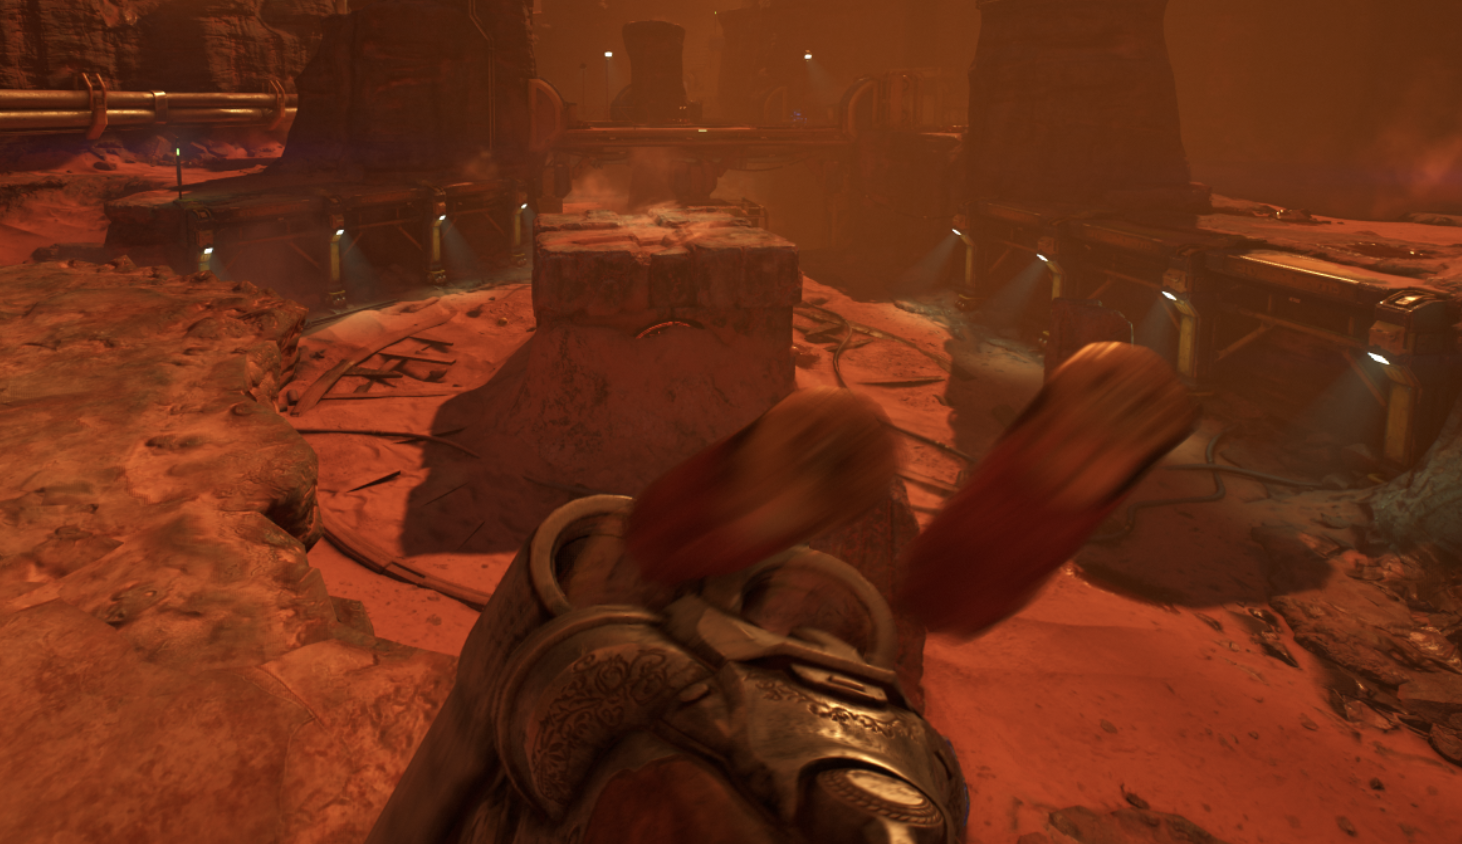
\includegraphics[width=\textwidth]{figures/doomblur1.png}
    \end{subfigure}
    \centering
    \begin{subfigure}[b]{0.8\textwidth}
        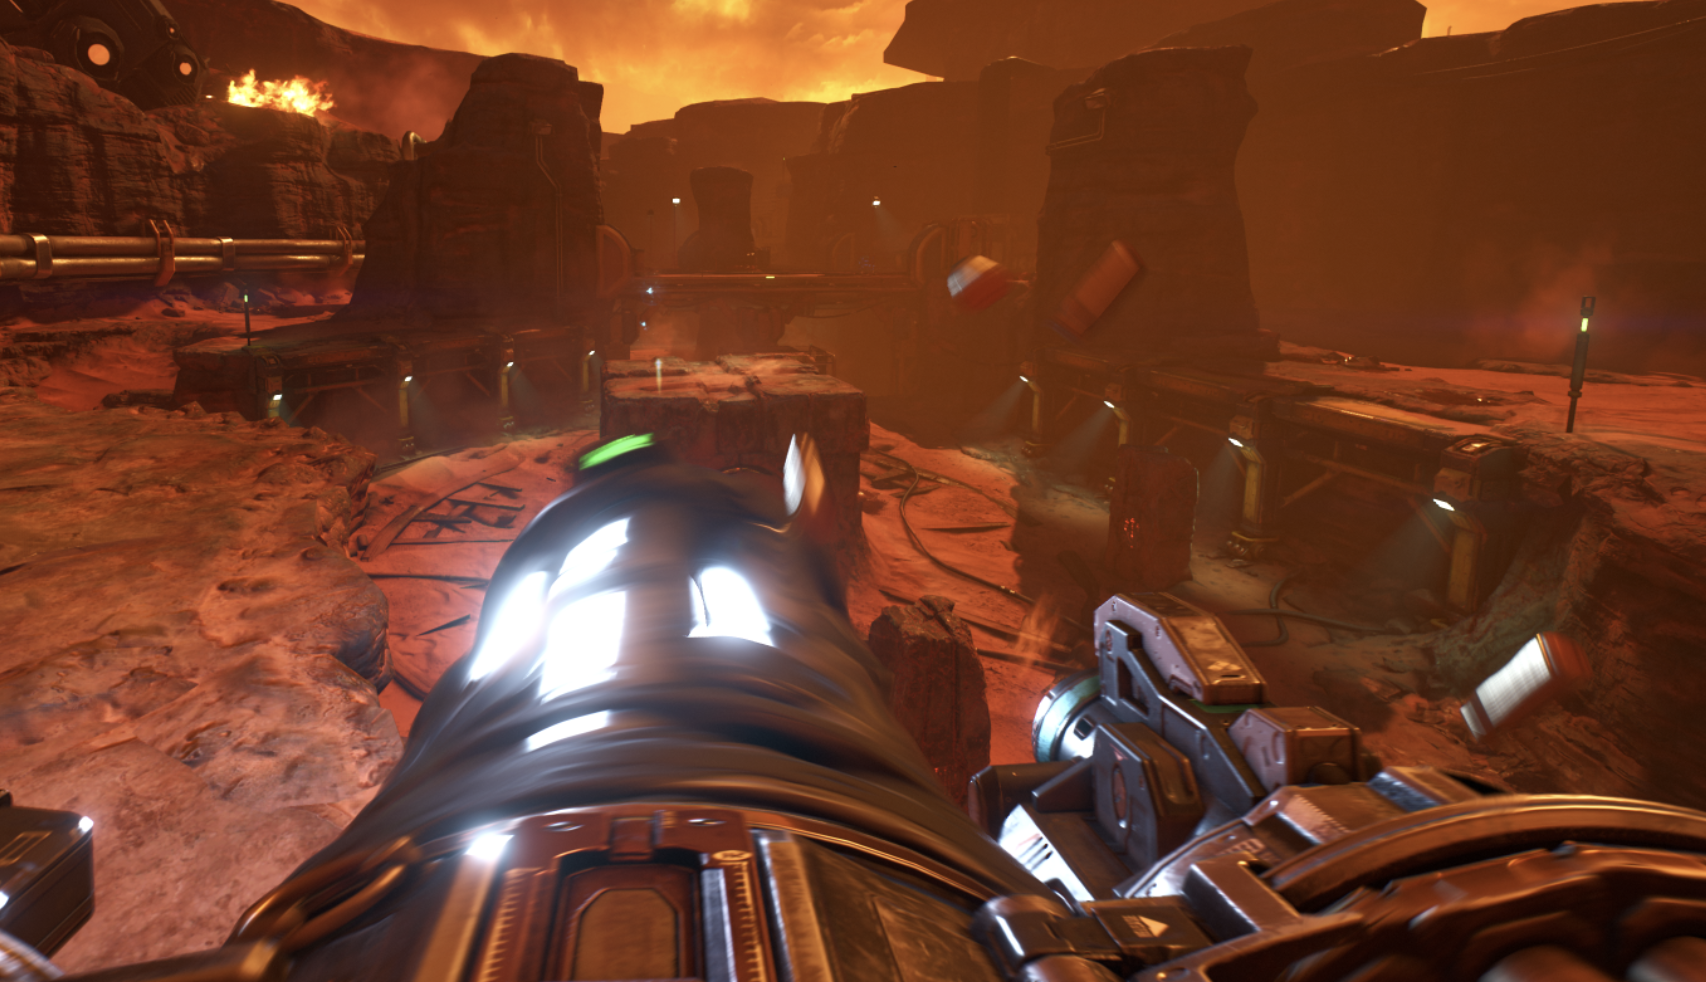
\includegraphics[width=\textwidth]{figures/doomblur2.png}
    \end{subfigure}
    \caption{Per object motion blur en Doom (2016)}
    \label{doomblur}
\end{figure}

\begin{figure}[!htbp]
    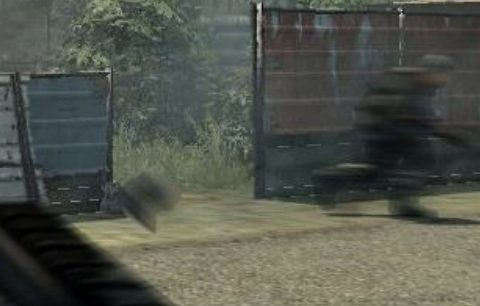
\includegraphics[width=.8\linewidth]{figures/crysisblur.png}
    \caption{Siluetas sobre objetos con blur en Crysis (2007)\cite{crysis}}
    \label{crysisblur}
\end{figure}

\begin{figure}[!htbp]
    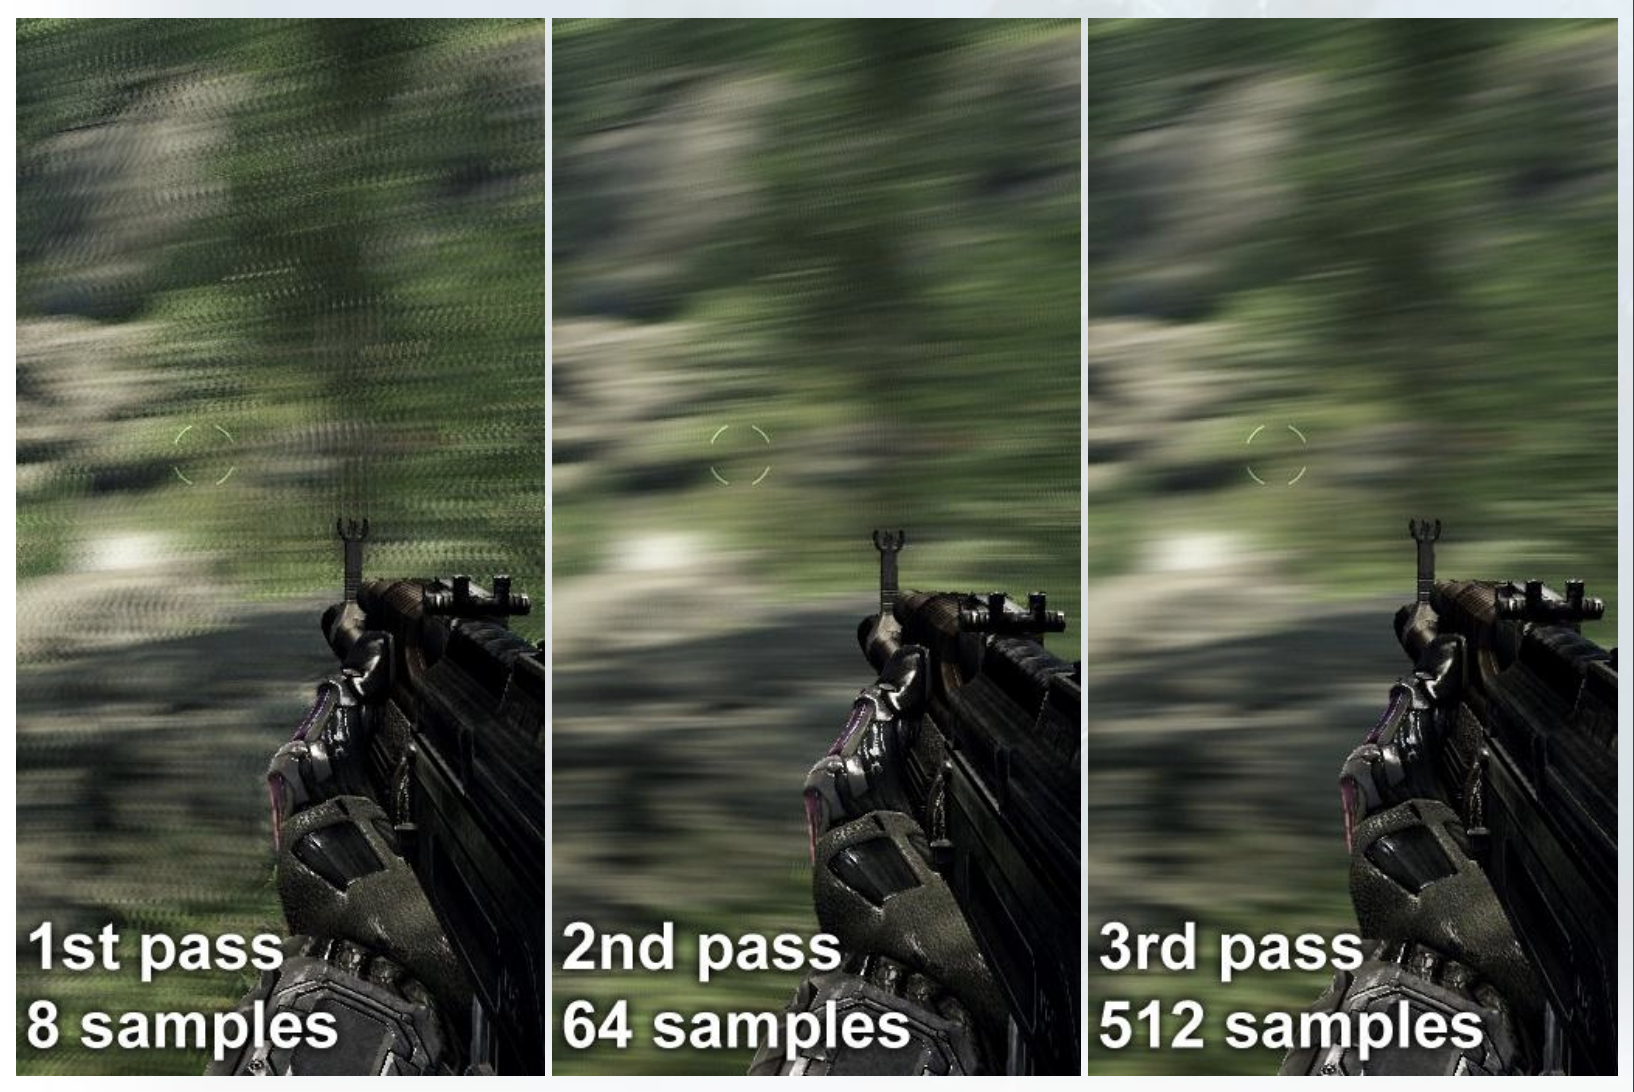
\includegraphics[width=.8\linewidth]{figures/blurringquality.png}
    \caption{Diferentes niveles de calidad de motion blur en Crysis (2007)\cite{crysis}}
    \label{blurringquality}
\end{figure}


\section{Tipos de Anti-aliasing}

El anti-aliasing es el conjunto de técnicas cuyo objetivo es el de disimular o eliminar las imperfecciones vistas anteriormente.

\subsection{Filtrado}
\label{filtros}

En gráficos raster (bidimensionales) el anti-aliasing se realiza mediante filtros. Para entender el filtrado en imágenes es necesario pensar en pixels no como pequeños cuadrados en una pantalla, si no en muestras de una función (normalmente 3 muestras, una por cada canal RGB)\cite{Smith95apixel}. Los filtros (o kernels) transforman las funciones para intentar suavizar los cambios bruscos de color.

En la figura~\ref{gls} se muestra una comparación de las diferentes formas en las que cada filtro interpola valores de una imagen con un solo canal. Cada punto representa la muestra de la función que se visualizará en la pantalla.

%\cite{resampling}

\begin{figure}[!htbp]
    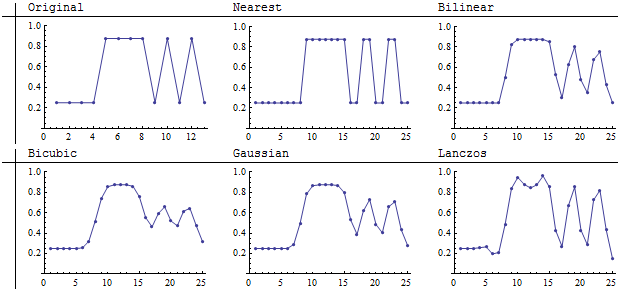
\includegraphics[width=\linewidth]{figures/Lw6ei.png}
    \caption{Comparación de interpolación usando diferentes filtros\cite{gis}}
    \label{gls}
\end{figure}

\begin{figure}[!htbp]
    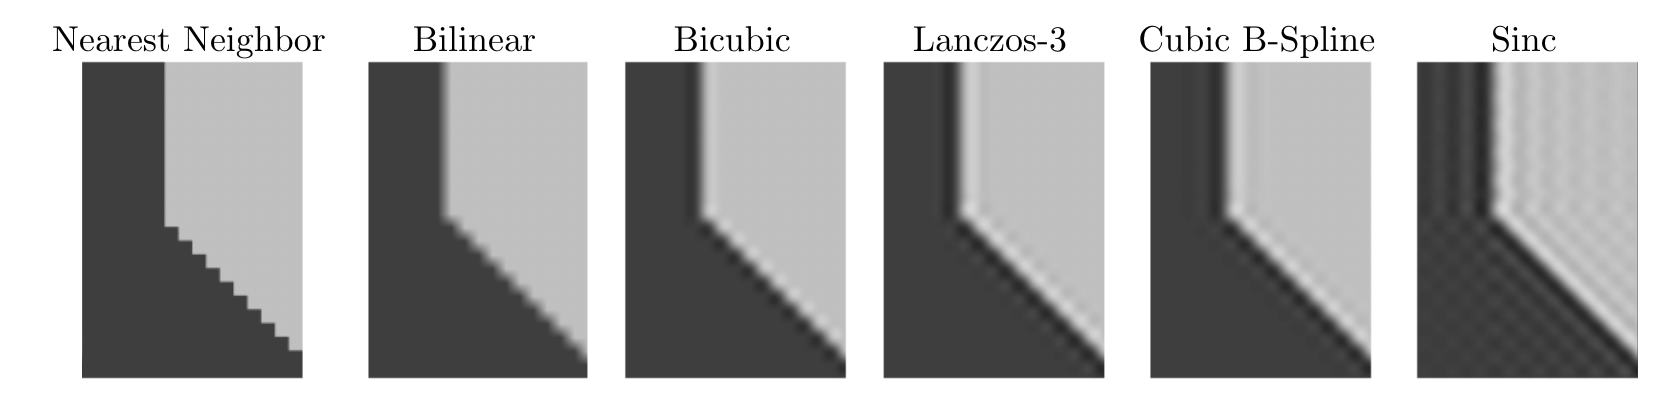
\includegraphics[width=\linewidth]{figures/comparison-filter.png}
    \caption{Comparación de resultados de diferentes filtros\cite{resampling2}}
\end{figure}

\subsection{Supersampling Anti-aliasing}

El supersampling consiste en minimizar el aliasing usando imágenes con una resolución mayor a la usada para su visualización (anti-aliasing espacial). Cada pixel en la pantalla será representado por más de un pixel en la imagen. Para el color final normalmente se hace la media del valor de los colores de los múltiples pixels\cite{Beets2000SupersamplingAA}.

Estas técnicas consumen más ancho de banda y memoria, ya que los buffers tienen que guardar más información por pixel que la imagen original.

La calidad del supersampling viene dado por la cantidad de samples por pixel y la técnica para saber que pixels usar en la imagen con mayor resolución para cada pixel de la pantalla.

En comparación a otras técnicas de anti-aliasing esta corrige aliasing de texturas (ver figuras \ref{ss1} y \ref{ss2}) y especular (ver figura \ref{specular}), además de aliasing de geometría. Esto se debe a que los subsamples los coge de en toda la escena.

\begin{figure}[!htbp]
    \centering
    \begin{subfigure}[b]{0.8\textwidth}
        
\includegraphics[width=\textwidth]{figures/ss1off.png}
        \caption{Anti-aliasing desactivado}
    \end{subfigure}
    \centering
    \begin{subfigure}[b]{0.8\textwidth}
        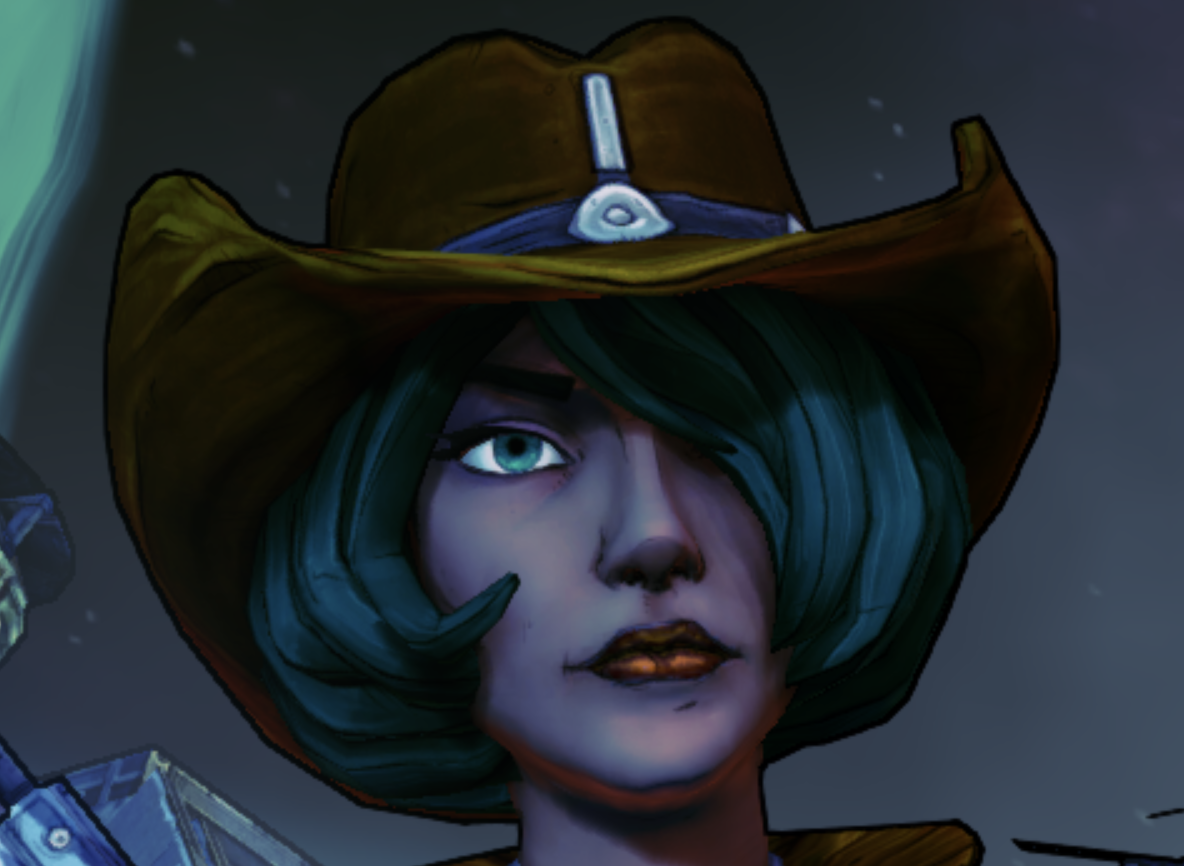
\includegraphics[width=\textwidth]{figures/ss1on.png}
        \caption{SSAA 4x}
    \end{subfigure}
    \caption{Resultados de SSAA en Borderlands 2}
    \label{ss1}
\end{figure}

\begin{figure}[!htbp]
    \centering
    \begin{subfigure}[b]{0.3\textwidth}
        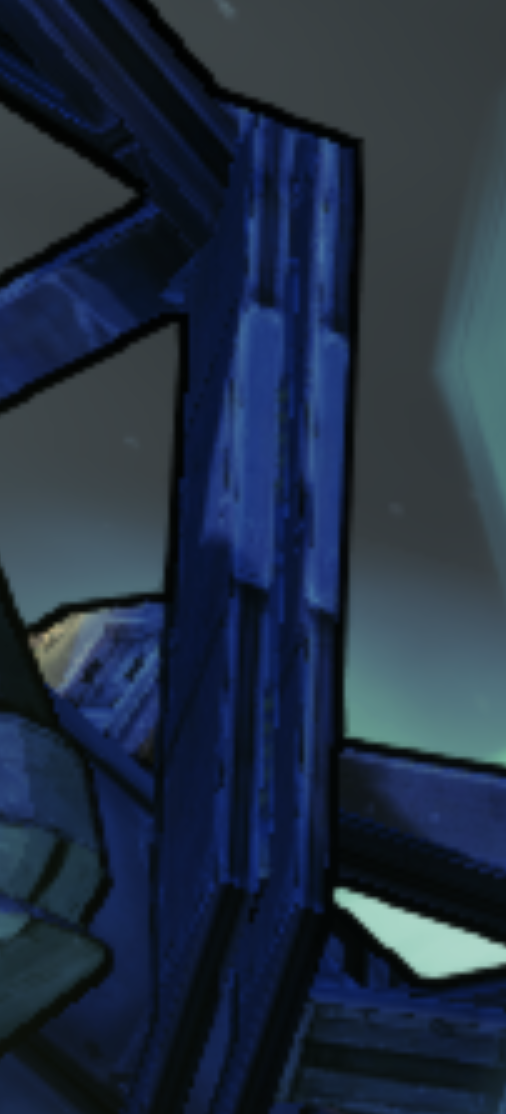
\includegraphics[width=\textwidth]{figures/ss2off.png}
        \caption{Anti-aliasing desactivado}
    \end{subfigure}
    \begin{subfigure}[b]{0.3\textwidth}
        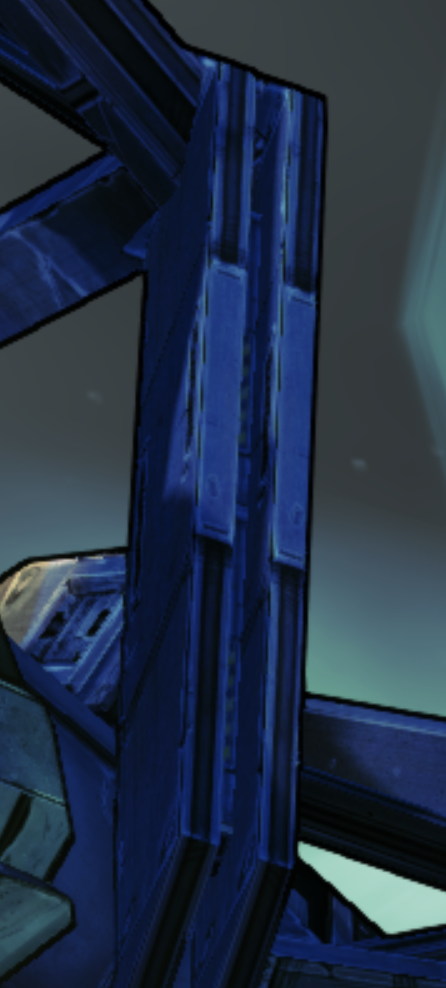
\includegraphics[width=\textwidth]{figures/ss2on.png}
        \caption{SSAA 4x}
    \end{subfigure}
    \caption{Resultados de SSAA en Borderlands 2}
    \label{ss2}
\end{figure}

\subsubsection{Ordered Grid Supersampling}

En esta técnica de supersampling la distribución de los samples es uniforme. Debido a la naturaleza regular de este patrón, los subpixels se encuentran situados en forma de dos columnas y dos filas. Para lineas muy planas, tanto en horizontal como vertical el anti-aliasing no será muy efectivo, ya que muy rápidamente tocará dos subpixels en fila o columna y hasta el final no tocará los otros subpixels, como se puede ver en la figura~\ref{ogss}.

Este efecto se puede reducir usando más samples, pero el impacto en el rendimiento será todavía mayor.

Desde 2014 Nvidia ha publicado una técnica llamada Dynamic Super Resolution\cite{960}, que consiste en renderizar software a mayor resolución y usar OGSS con un filtro de blur gaussiano. En 2015 AMD implementó una técnica similar llamada Virtual Super Resolution.

\begin{figure}[!htbp]
    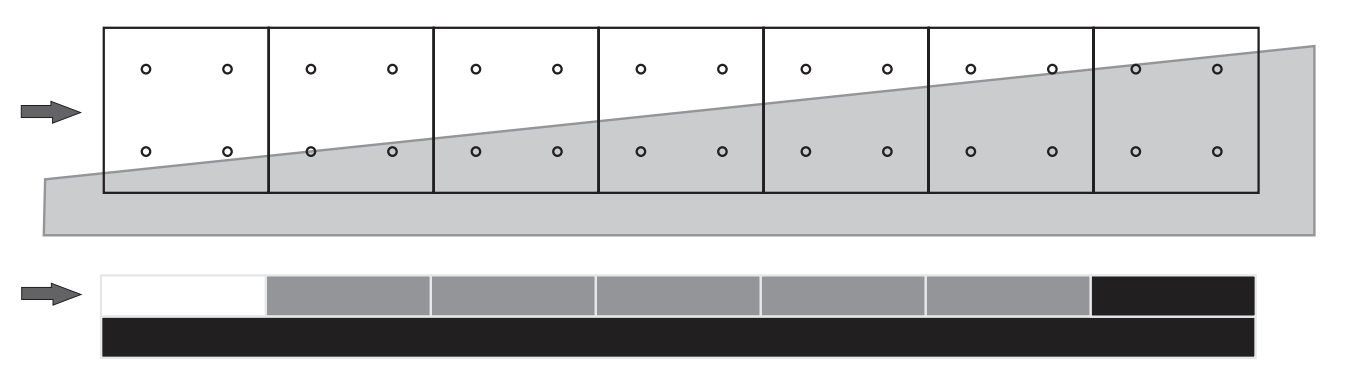
\includegraphics[width=\linewidth]{figures/ogss.png}
    \caption{Ordered Grid Super-Sampling\cite{Beets2000SupersamplingAA}}
    \label{ogss}
\end{figure}

\subsubsection{Rotated Grid Supersampling}

En el caso del RGSS se cambia el lugar de los subsamples para minimizar la cantidad de columnas y filas. La distribución sigue siendo uniforme, pero el problema del aliasing en lineas muy planas se soluciona, como se puede apreciar en la figura~\ref{rgss}, sin tener que recurrir a aumentar de manera significativa el numero de subsamples.

\begin{figure}[!htbp]
    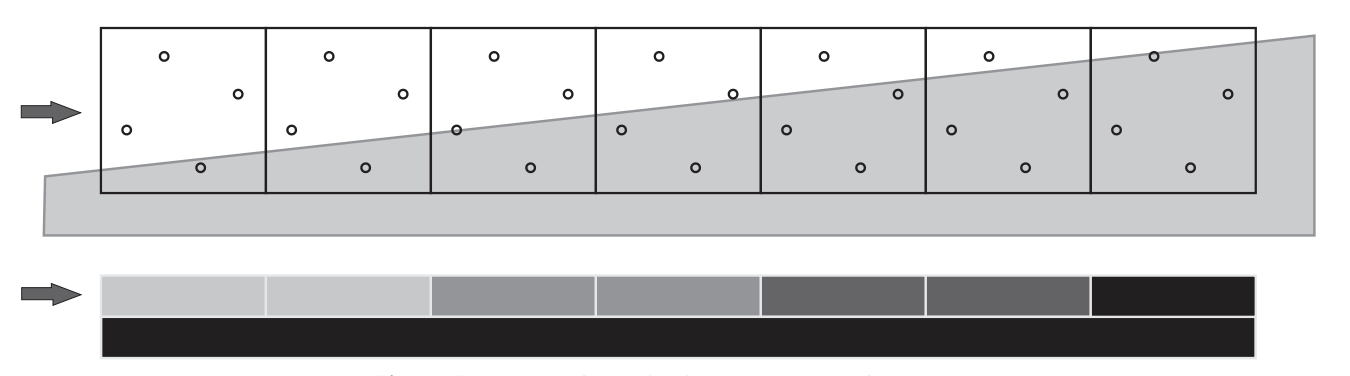
\includegraphics[width=\linewidth]{figures/rgss.png}
    \caption{Rotated Grid Super-Sampling\cite{Beets2000SupersamplingAA}}
    \label{rgss}
\end{figure}

\subsubsection{Quincunx Supersampling}

Este patrón es interesante como técnica de supersampling ya que usa subsamples localizados en las esquinas de los pixels, lo que permite reutilizar varios subsamples entre pixels (figura~\ref{fig:quincunx}). Esto permite una calidad similar a la de un anti-aliasing 4x pero con un coste computacional de un supersampling 2x. Aún así al reutilizar subsamples produce resultados algo más borrosos que otros métodos.

Aunque este patrón se pueda usar para supersampling Nvidia lo implementó en hardware desde la GeForce 3\cite{hraa} para acelerar el calculo de su multisampling. Sony al utilizar una GPU de Nvidia en la PS3 también disponía de esta tecnología en la consola.

\begin{figure}[!htbp]
    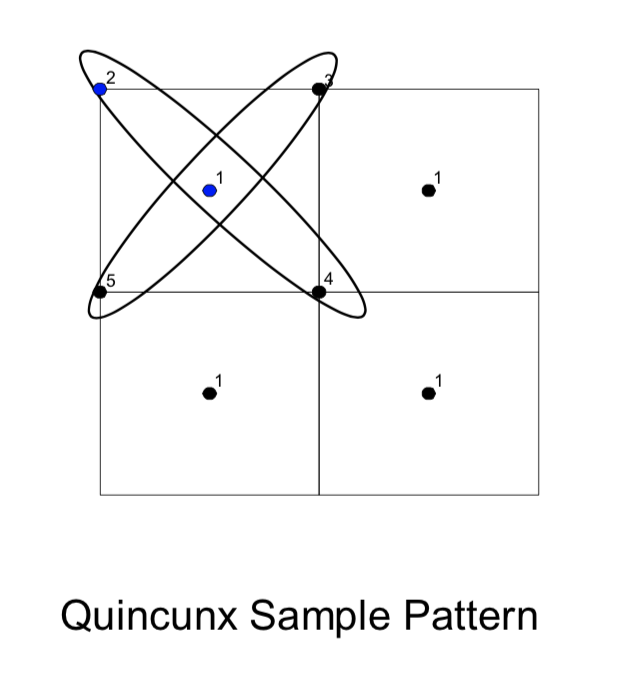
\includegraphics[width=.5\linewidth]{figures/quincunx.png}
    \caption{Quincunx Pattern\cite{hraa}}
    \label{fig:quincunx}
\end{figure}

\subsection{Multisampling}

El multisampling es una optimización del supersampling. Se siguen usando subpixels, pero en vez de resolver el color para cada subpixel el color se resuelve una única vez por pixel. Después de resolver el color se calcula el stencil buffer y depth buffer con subpixels, y dependiendo de la cantidad de subpixels que estén contenidos dentro del triangulo se usará un porcentaje del valor del color calculado. Esto reduce drásticamente el impacto en el rendimiento de la aplicación, ya que solo hay que acceder una vez por pixel a la textura, pero solo soluciona aliasing en los bordes de la geometría\cite{nvidiamsaa}\cite{msaa}.

En el centro de un polígono todos los subpixels van a estar contenidos dentro, pero el color solo se calcula una vez (por ejemplo en el centro del pixel), por lo que se usará el 100\% del color, pero puede contener aliasing. En cambio, en los bordes, algún subpixel estará fuera de la geometría, por lo que se usará un porcentaje del color calculado, suavizando el borde.

Otra de las desventajas del multisampling anti-aliasing es que, tradicionalmente, no se puede usar en motores con deferred shading. Debido a que el calculo del color final de cada pixel se realiza en un pixel shader posterior al cálculo del g-buffer (figura \ref{gbuffer}), al hacer el resolve del mutisampling no está lista toda la información necesaria. Desde \Gls{opengl} 3.2 y Direct3D 10.1 esto ha cambiado gracias al explicit multisampling\cite{textureMultisample}. La creación del g-buffer ahora se puede realizar usando texturas multisampled y al calcular la luz se puede acceder a los subsamples mediante la función texelfetch. Si se realiza de esta forma hay que sacrificar la creación automática de mipmaps y filtrado de texturas, aunque siempre se pueden implementar manualmente en shaders. Aún así muchos desarrolladores han optado por usar post-processing anti-aliasing al usar deferred shading.

\begin{figure}[!htbp]
    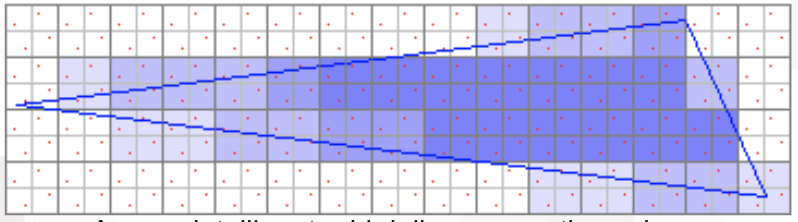
\includegraphics[width=.8\linewidth]{figures/msaasample.png}
    \caption{Multisampling}
    \label{msaasample}
\end{figure}

\begin{figure}[!htbp]
    \centering
    \begin{subfigure}[b]{0.8\textwidth}
        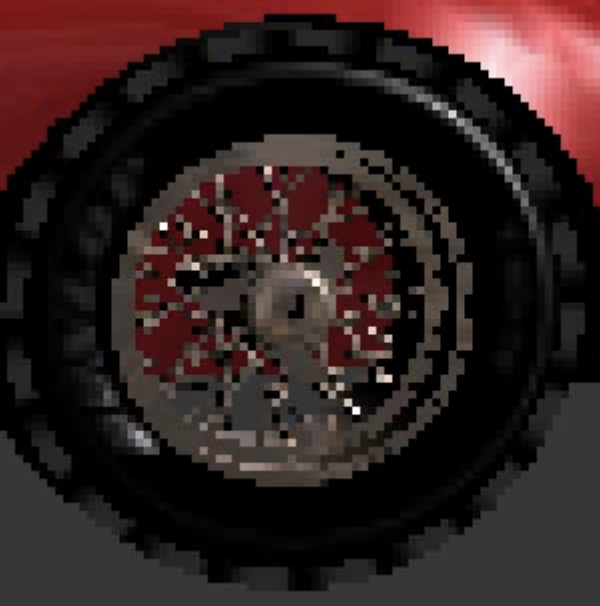
\includegraphics[width=\textwidth]{figures/msaaoff.png}
        \caption{Anti-aliasing desactivado}
    \end{subfigure}
    \centering
    \begin{subfigure}[b]{0.8\textwidth}
        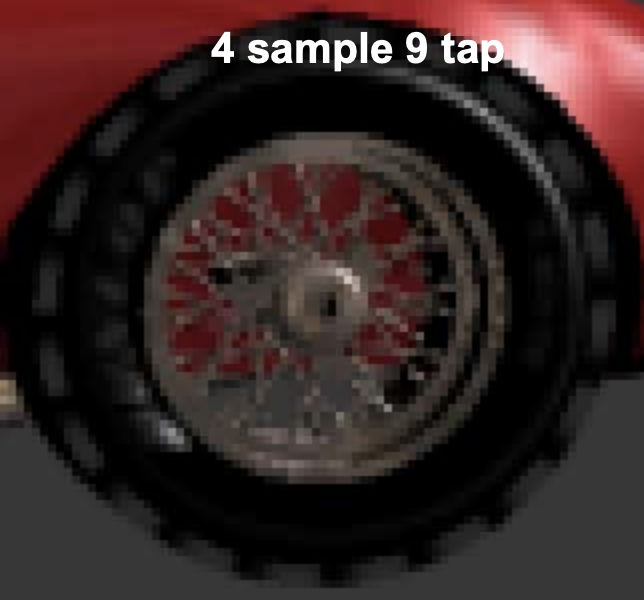
\includegraphics[width=\textwidth]{figures/msaa.png}
        \caption{MSAA 4x}
    \end{subfigure}
    \caption{Resultados del MSAA}
    \label{msaares}
\end{figure}

\begin{figure}[!htbp]
    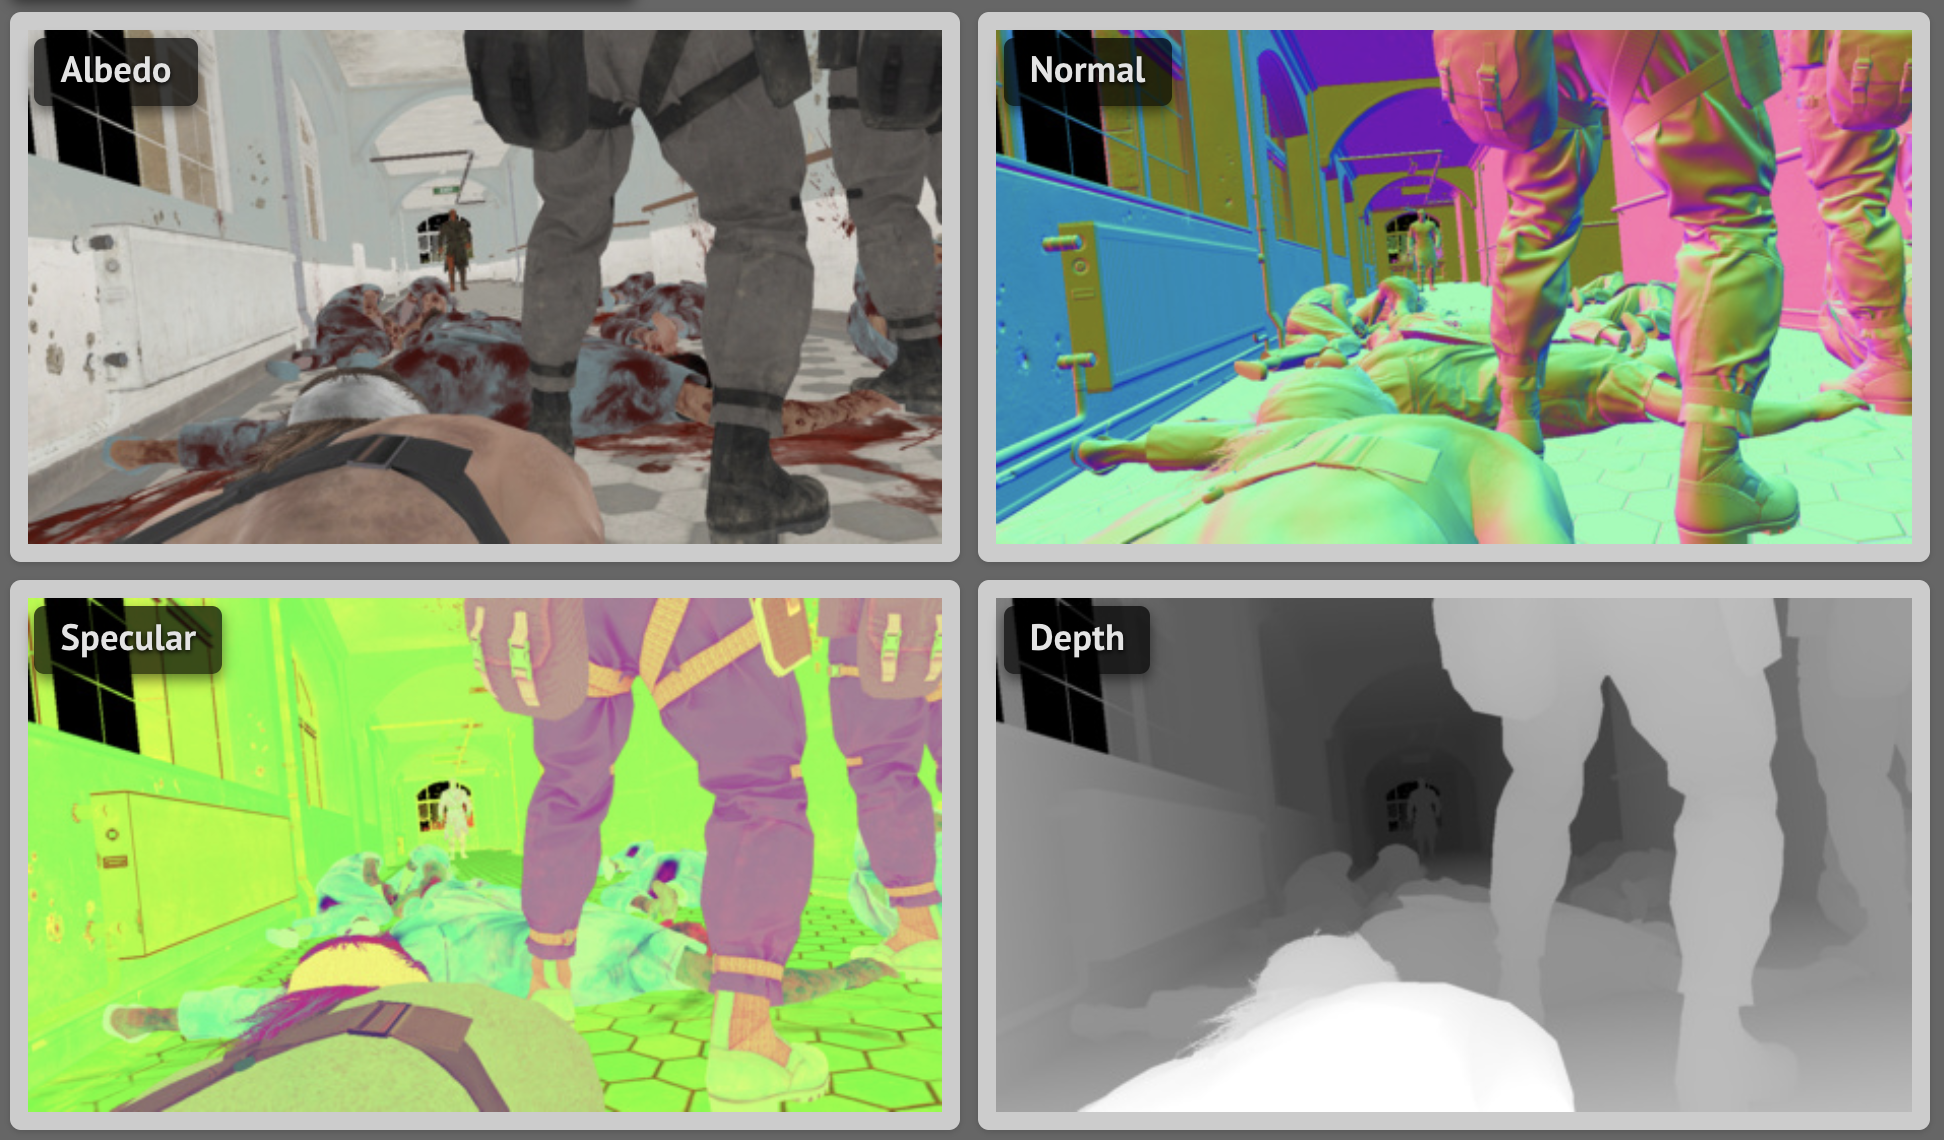
\includegraphics[width=\linewidth]{figures/gbuffer.png}
    \caption{Generación de G-Buffer en Metal Gear Solid V\@: The Phantom Pain\cite{analysismgsv}}
    \label{gbuffer}
\end{figure}

\subsection{Post Processing Anti-aliasing}

Este tipo de anti-aliasing ha ganado popularidad durante los últimos años, debido en parte al uso del deferred shading en los últimos motores gráficos. Los algoritmos presentados a continuación se pueden considerar filtros de rasters, como los de la sección~\ref{filtros}, pero están pensados para ser usados en motores gráficos. Además, en muchos casos, usan información que no está presente en la textura final, como pueden ser texturas de profundidad o vectores de movimiento,

\subsubsection{Fast Approximate Anti-aliasing}

El FXAA\cite{FXAA} es un sistema de anti-aliasing de post procesado desarrollado por NVIDIA\@. Se implementa como un único pixel shader y tiene diferentes niveles de calidad. El impacto en su rendimiento es muy bajo en comparación a métodos con resultados similares (inferior a 1ms).

Recibe la imagen final en formato RGB y la transforma en valores de luminancia por pixel. Usando el contraste entre pixels adyacentes detecta los bordes (figura \ref{fxaaedge}). Cada borde es clasificado como horizontal o vertical. Dependiendo de los valores de luminancia y orientación de cada borde se aplica un pequeño offset para cada pixel y se hace un resampling para calcular un nuevo color que reduzca el aliasing\cite{FXAA}\cite{fxaa2}.

\begin{figure}[!htbp]
    \includegraphics[width=\linewidth]{figures/fxaaedge.png}
    \caption{Detección de bordes usando valores de luminancia\cite{fxaa2}}
    \label{fxaaedge}
\end{figure}

\begin{figure}[!htbp]
    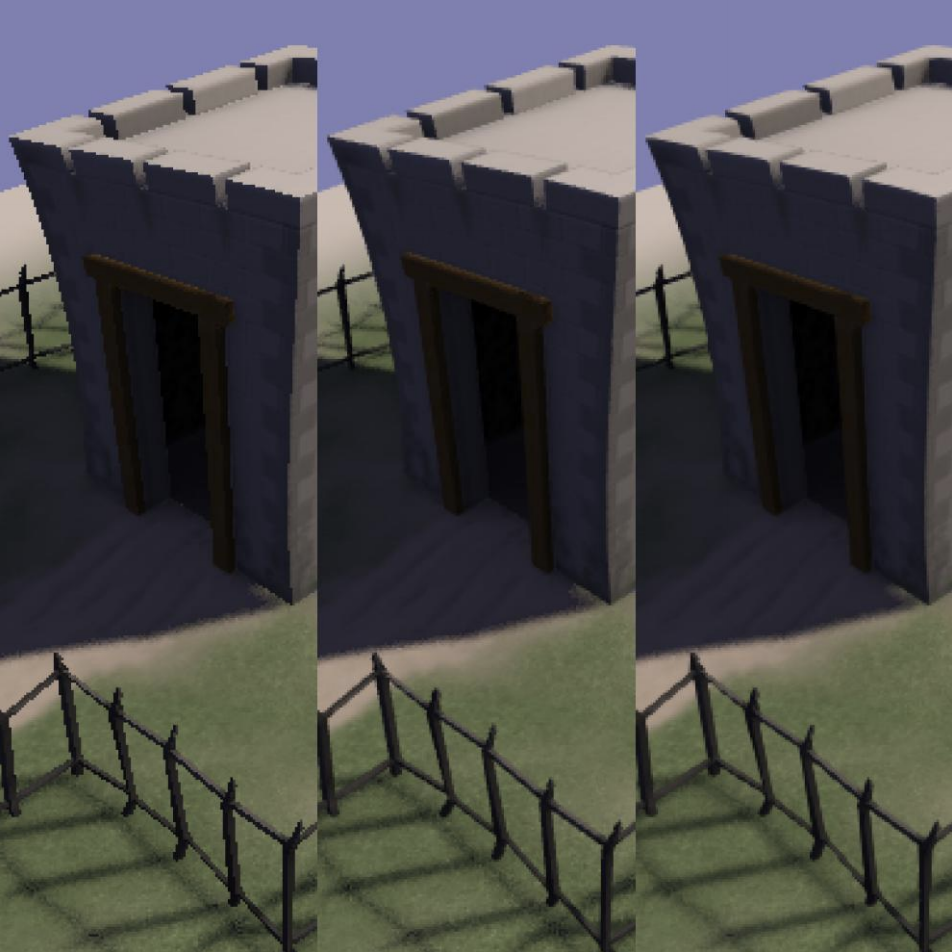
\includegraphics[width=.8\linewidth]{figures/fxaacomparison.png}
    \caption{Escena con AA off, MSAA 4x y FXAA }
    \label{fxaacomparison}
\end{figure}

\subsubsection{Morphological Anti-aliasing}

El MLAA\cite{Reshetov:2009:MA:1572769.1572787} se basa en buscar los bordes discontinuos basándose en los colores de los pixels. Consigue discernir entre bordes con forma de $U$, $Z$ y $L$. Finalmente mezclará los bordes con los colores de los pixels adyacentes.

\begin{figure}[!htbp]
    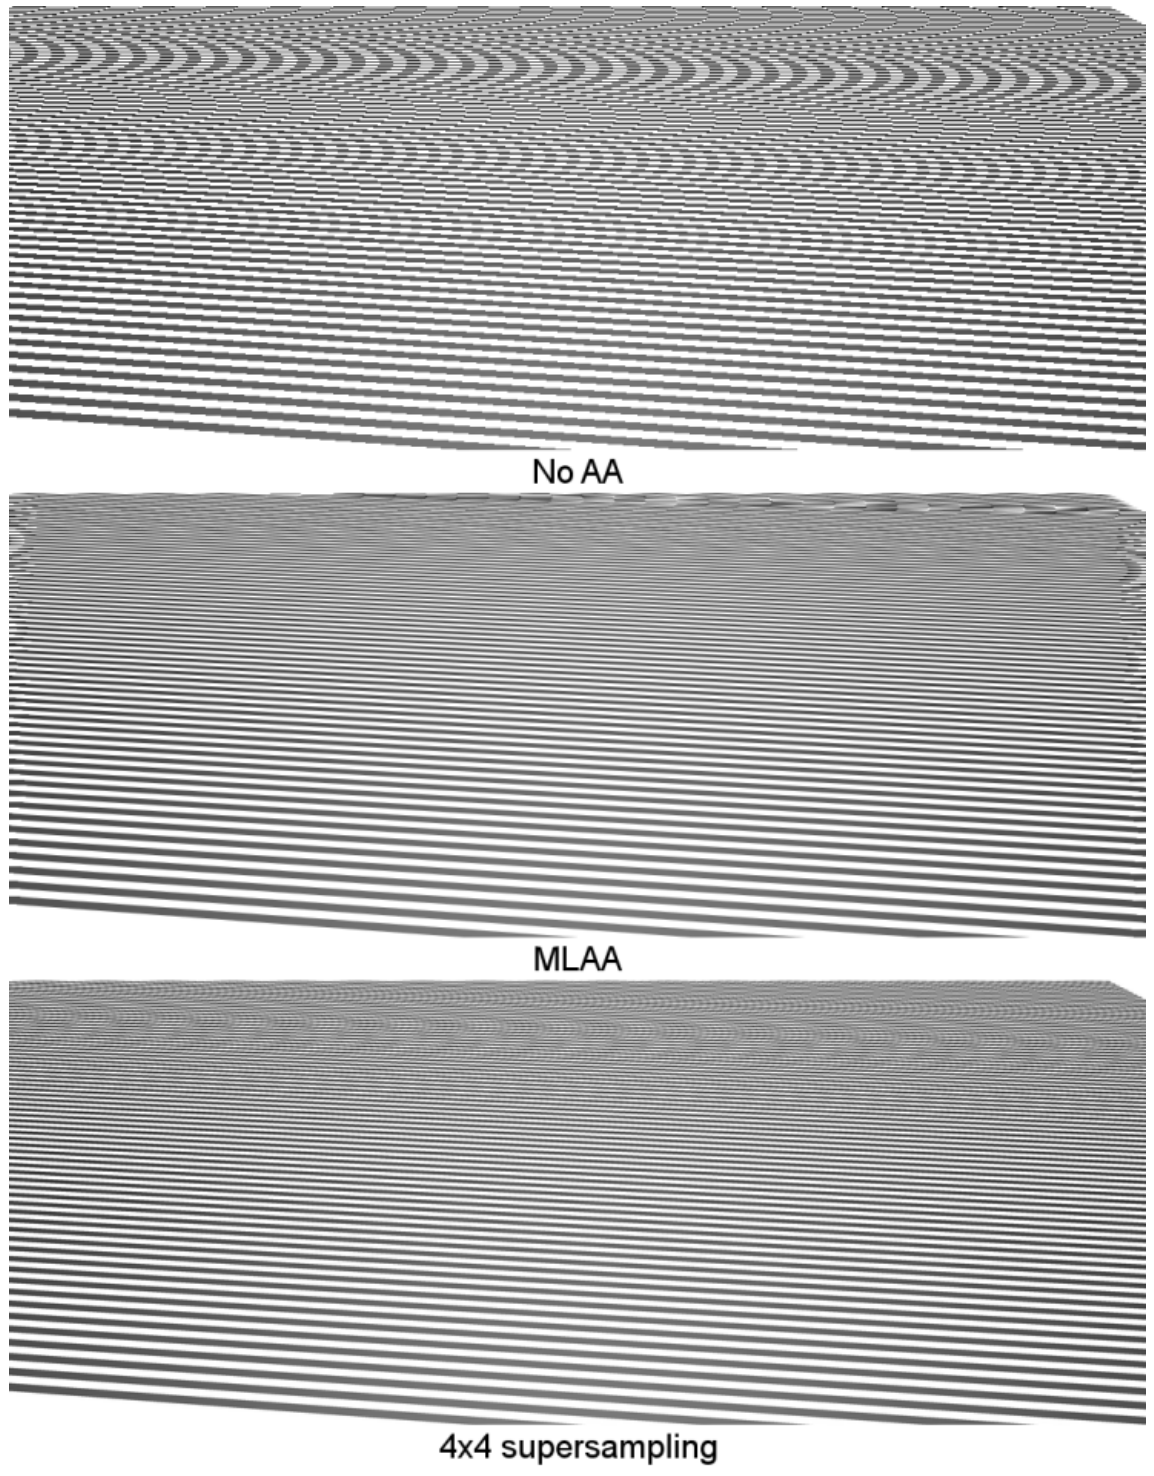
\includegraphics[width=.8\linewidth]{figures/mlaacomparison.png}
    \caption{MLAA en blanco y negro}
    \label{mlaacomparison}
\end{figure}

\begin{figure}[!htbp]
    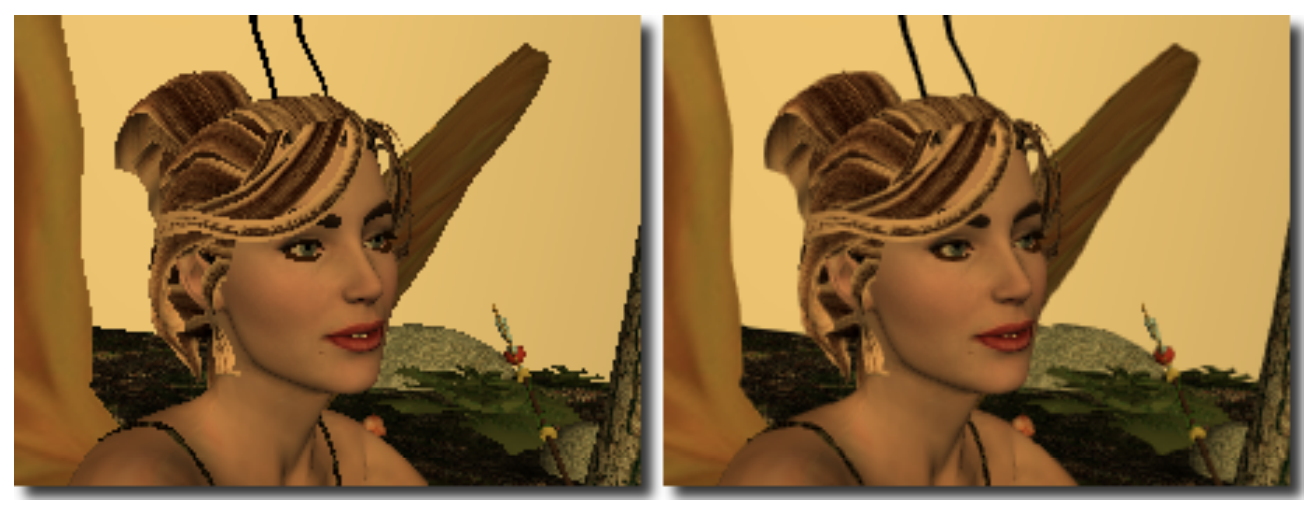
\includegraphics[width=\linewidth]{figures/mlaares.png}
    \caption{MLAA con color}
    \label{mlaacomparison}
\end{figure}

\subsubsection{Enhanced Subpixel Morphological Anti-aliasing}

El SMAA\cite{Jimenez:2012:SES:2318858.2318861} se basa en MLAA, pero aplicando unas variaciones con el fin de mejorar el resultado final. La calidad de imagen es más elevado, pero tiene un coste computacional algo mayor.

Las variaciones con respecto a MLAA son:

\begin{itemize}
    \item Consigue clasificar más formas de bordes, incluidas las lineas diagonales
    \item Usa contraste local en vez de color como métrica de comparación de valores entre pixels
    \item Puede funcionar con más de un sample por pixel, junto a un supersampling tradicional
\end{itemize}

En la figura \ref{halo1} se puede ver la calidad del resultado final. Como con el resto de técnicas de anti-aliasing de post-procesado, aunque la aplicación no tenga soporte nativo para SMAA (como es el caso de Halo 1) se puede inyectar mediante software, gracias a que se ejecuta como una pasada final a la imagen.

\begin{figure}[!htbp]
    \centering
    \begin{subfigure}[b]{0.8\textwidth}
        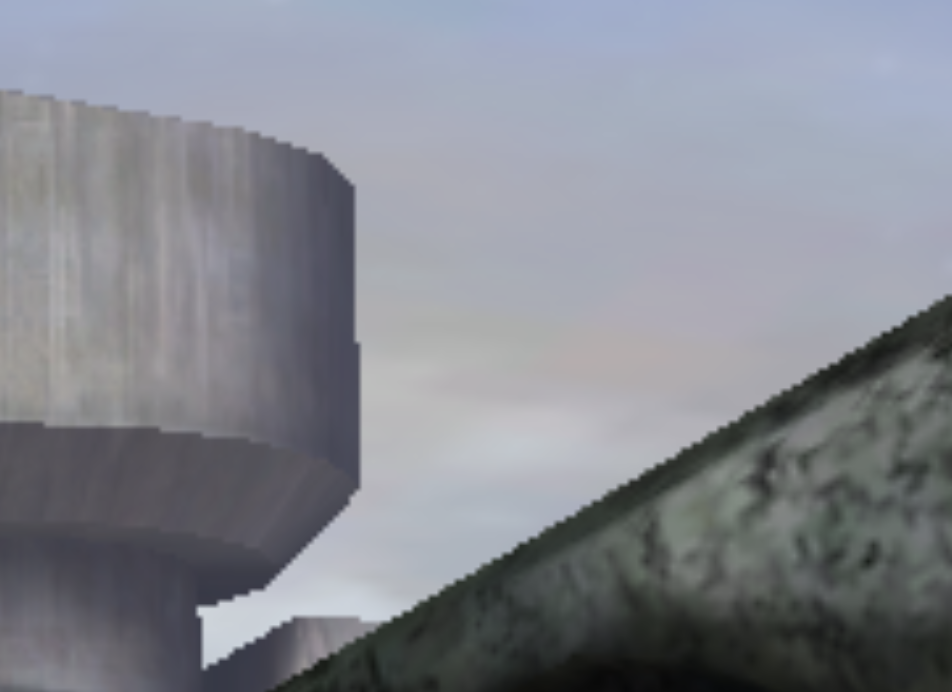
\includegraphics[width=\textwidth]{figures/smaaOFF.png}
        \caption{Anti-aliasing desactivado}
    \end{subfigure}
    \centering
    \begin{subfigure}[b]{0.8\textwidth}
        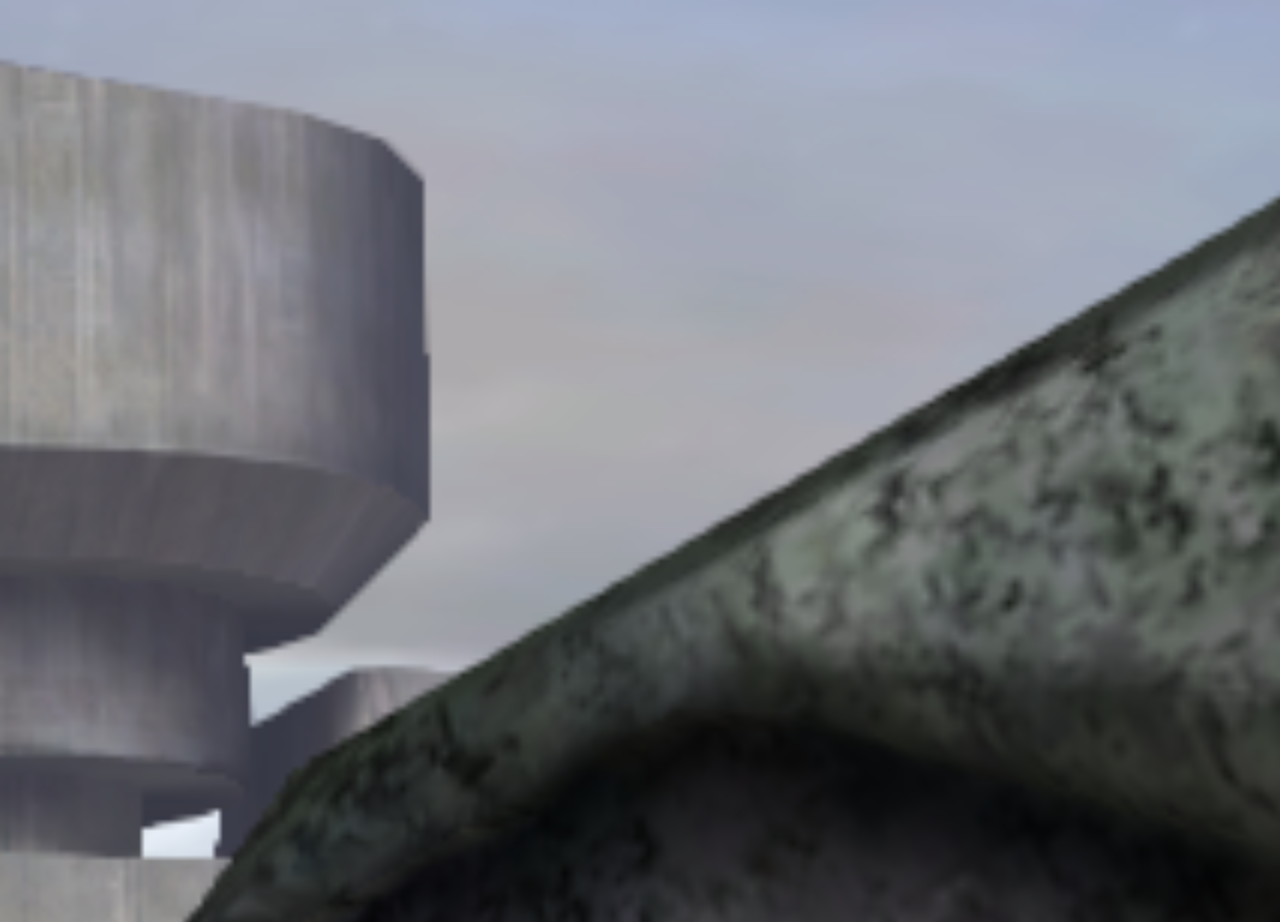
\includegraphics[width=\textwidth]{figures/smaaON.png}
        \caption{SMAA}
    \end{subfigure}
    \caption{Comparación de antialiasing en Halo 1 (2001)}
    \label{halo1}
\end{figure}

\subsection{Temporal Anti-aliasing}

El temporal anti-aliasing es un tipo de anti-aliasing de post procesado, pero que amortiza el coste computacional usando múltiples samples en múltiples frames. Esto presenta unas complicaciones a la hora de escoger samples en frames anteriores en imágenes no estáticas.

Su implementación y resultados se explican en más detalles en los siguientes capítulos.

\subsection{Machine Learning Anti-aliasing}

Están empezando a aparecer técnicas que usan algoritmos de machine learning (como redes neuronales profundas) para generar una imagen con mayor calidad a la original. Este tipo de problemas son ideales para algoritmos de machine learning, ya que es fácil conseguir datos con los que entrenar las redes y no existe ninguna solución algorítmica ideal que se pueda usar en tiempo real\cite{Huang-CVPR-2015}\cite{5459271} (ver figura \ref{superres}).

Nvidia, desde la arquitectura Turing, ha comenzado a explotar estas técnicas para mejorar la calidad del anti-aliasing\cite{turingwhitepaper}. Esta arquitectura cuenta con hardware especifico que acelera tareas de deep learning. Nvidia entrenará redes neuronales para cada software en cuestión con imágenes reales usando supersampling x64. La red ajustará sus valores en cada iteración del entrenamiento hasta llegar a un nivel satisfactorio de calidad. Estas redes entrenadas se distribuirán a los usuarios de tarjetas Turing.

\begin{figure}[!htbp]
    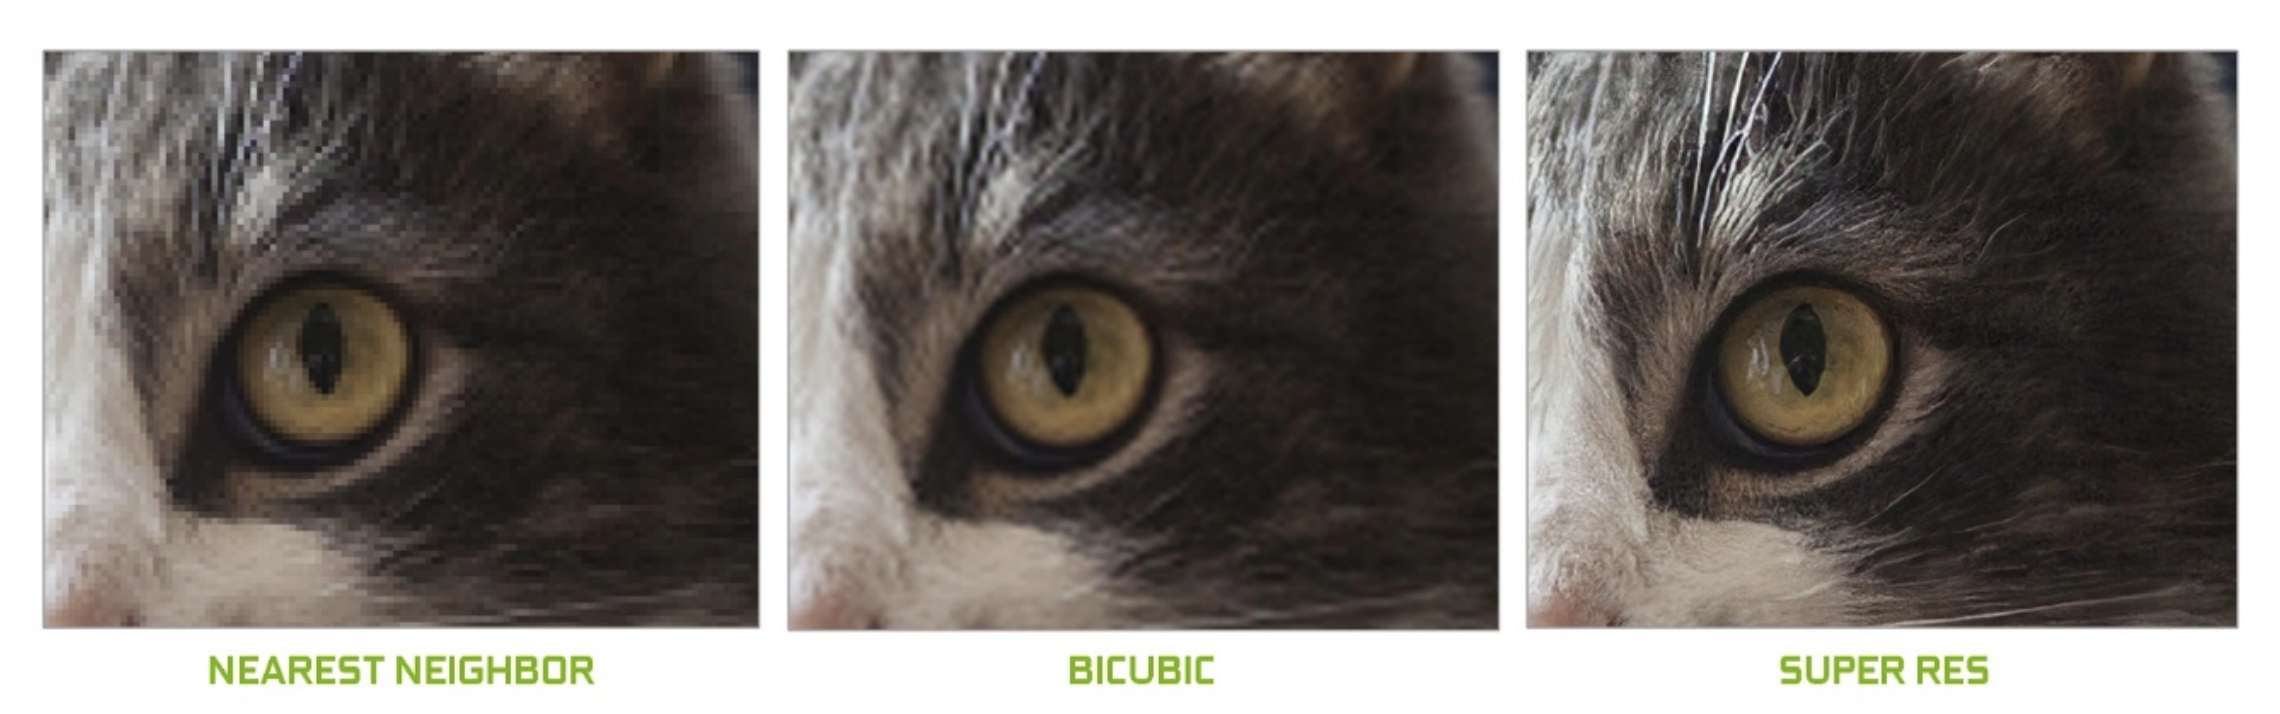
\includegraphics[width=\linewidth]{figures/superres.png}
    \caption{Super Res\cite{turingwhitepaper}}
    \label{superres}
\end{figure}

\begin{figure}[!htbp]
    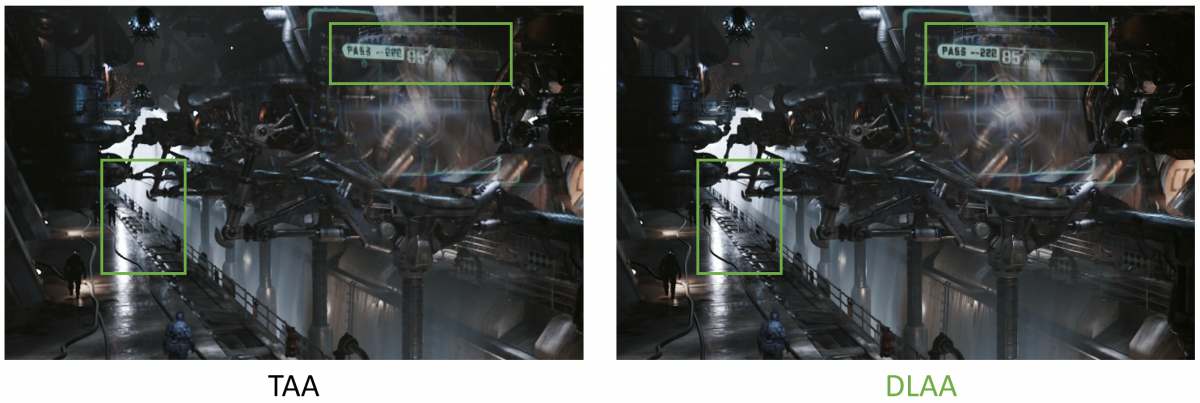
\includegraphics[width=\linewidth]{figures/dlss.png}
    \caption{DLSS\cite{turingwhitepaper}}
    \label{fig:dlss}
\end{figure}

\chapter{Desarrollo}

Para este proyecto se ha integrado un sistema de anti-aliasing temporal en un motor de gráficos 3D que usa \Gls{opengl} como API gráfica. Su implementación se ha realizado mediante shaders GLSL y código C++ 14. El motor gráfico sobre el que se ha implementado es propio y se ha desarrollado durante el Máster Universitario en Computación Gráfica y Simulación de U-Tad en el curso 2017--2018.

De manera general, el motor ha tenido que ser modificado para incluir funcionalidad de post-procesado de imágenes mediante Frame Buffer Objects, métodos para la realización del jitter, y shaders que calculan el anti-aliasing en sí. No se ha empleado ninguna funciona de anti-aliasing que proporciona \Gls{opengl} de manera automática, como el uso de texturas GL\_TEXTURE\_2D\_MULTISAMPLE\@.

En primer lugar es necesario poder guardar el resultado del frame anterior, desplazar la cámara ligeramente cada frame (creando subsamples únicos en cada frame), calcular el desplazamiento de la cámara, mezclar colores del frame anterior al actual, y finalmente aplicar un filtro de sharpening.

\section{History Buffer}

Debido a la necesidad de combinar varias texturas de frames anteriores, para calcular el anti-aliasing de un frame $n$ es necesario tener acceso al frame $n_{-1}$. Aún usando más de 2 subsamples solo es necesario guardar el último, siempre y cuando tenga el anti-aliasing ya incluido.

También se puede optar por guardar $n$ frames para $n$ subsamples y combinarlos en un pixel shader, pero esto ocupa mucha más memoria y es impráctico.

Para esto es necesario crear un FBO y guardar el resultado de la textura como variable, que durante el siguiente frame será pasada al shader como un uniform sampler2D, y así poder acceder a sus pixels.

\begin{minted}{cpp}
\end{minted}

\section{Jitter}

En primer lugar es necesario elegir los subsamples a usar en cada frame. Recordemos que en vez de calcular varios subsamples en cada frame, el temporal anti-aliasing calcula un solo sample por frame. Cada frame cambiará el lugar del subsample a calcular. Gracias a que solo se calcula un subsample por frame el impacto en el rendimiento será mucho menor al del supersampling tradicional.

Para elegir los subsamples se pueden usar los grids vistos anteriormente en la sección sobre supersampling\cite{unrealtaa}. Aún así en la práctica se suelen usar secuencias de Halton (figura~\ref{halton}).

Las secuencias de Halton proporcionan una baja discrepancia, lo que significa que no se van crear clusters ni en espacio ni en tiempo. Esto proporciona una calidad de subsamples muy alta por lo que la calidad del anti-aliasing puede ser muy elevado. Siempre que esté bien implementado los resultados serán mejores que los del anti-aliasing por hardware implementado hasta ahora\cite{unrealtaa}.

Una vez se ha calculado la secuencia de Halton en cada frame se alterará la matriz $MVP$ para mover el sample al lugar del subsample que toque en ese frame. Este lugar cambiará cada vez que se genera un nuevo frame.

En este punto si viésemos la imagen seguiríamos notando el aliasing y la imagen parecería que estuviera vibrando ligeramente.

\begin{figure}[!htbp]
    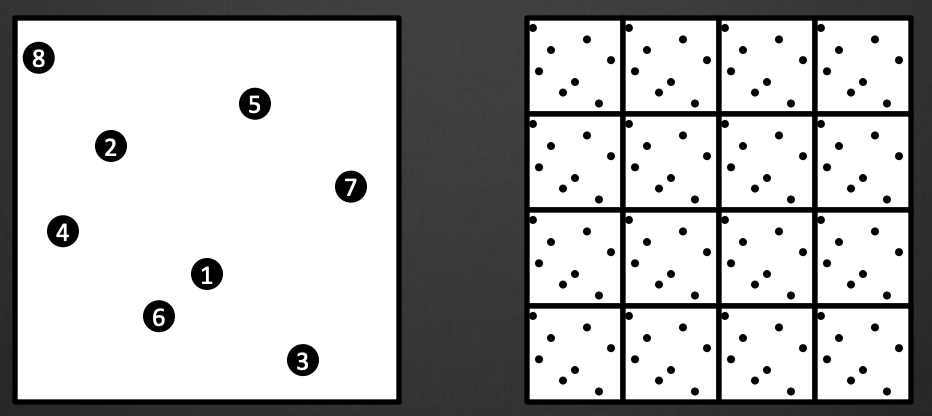
\includegraphics[width=\linewidth]{figures/halton.png}
    \caption{Jitter con secuencia Halton}
    \label{halton}
\end{figure}

\begin{minted}{cpp}
float Halton(int Index, int Base) {
    float Result = 0.0f;
    float InvBase = 1.0f / Base;
    float Fraction = InvBase;
    while (Index > 0)
    {
        Result += (Index % Base) * Fraction;
        Index /= Base;
        Fraction *= InvBase;
    }
    return Result;
}
\end{minted}

\section{Motion Vectors}

El segundo paso para la implementación del temporal anti-aliasing consiste en la creación de un velocity buffer. Este buffer contendrá una textura fp16 con dos canales de color (rojo y verde) donde cada pixel representa un vector.

Ese vector representa cuanto se ha movido un pixel del frame actual ($n$) al anterior ($n_{-1}$). Cada pixel viene definido por sus posiciones en $x$ e $y$. Para calcular el velocity buffer se usa su posición actual $C = x_{n}y_{n}$ y su posición previa $P = x_{n_{-1}}y_{n_{-1}}$. En el velocity buffer se almacena $\vec{CP}$, como se ilustra en la figura \ref{vec}.

\begin{figure}[!htbp]
    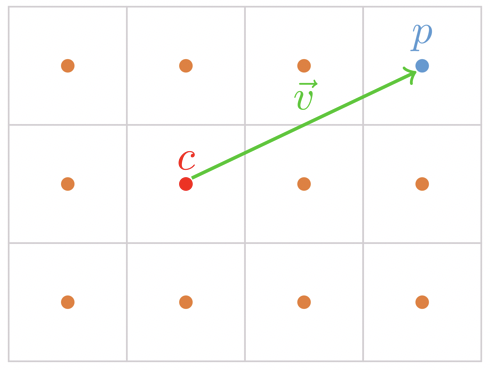
\includegraphics[width=.5\linewidth]{figures/vec.png}
    \caption{$\vec{CP}$\cite{filmicsmaa}}
    \label{vec}
\end{figure}

Para la creación del velocity buffer en una escena dinámica es imprescindible saber no solo el movimiento de cámara del frame anterior, si no como se han movido los objetos. Esto se complica si hay objetos translucidos como ventanas, o que reflejan luz como los espejos\cite{uncharted4}.

En este proyecto se ha optado por usar el algoritmo descrito en el capítulo 27 de GPU Gems 3\cite{Nguyen:2007:GG:1407436} para su implementación. Solo es necesario usar un pixel shader junto al history buffer, el depth buffer y las matrices $VP_{n}$ y $VP_{n_{-1}}$. La ventaja de este algoritmo es que no depende mucho de la implementación del motor. Nvidia incluye una librería que hace estos calculas en el SDK PostWorks\cite{postworks} (usado para la implementación de \GLS{TXAA}).

Otra posibilidad es computar la velocidad durante una segunda pasada del vertex shader de cada polígono, pero dependiendo de su implementación puede resultar algo más lenta. Aún así debería resultar en vectores más precisos y en algunas ocasiones será necesario\cite{asscreed}.

\begin{minted}{glsl}
#version 330 core
uniform sampler2D depthTexture;

in vec2 TexCoords;
uniform mat4 VP;
uniform mat4 PrevVP;

out vec4 velocity;

void main() {
    float zOverW = texture2D(depthTexture, TexCoords).r
                   * 2.0f - 1.0f;

    vec4 H = vec4(TexCoords.x * 2.0f - 1.0f,
                  (1.0f - TexCoords.y) * 2.0f - 1.0f,
                  zOverW, 1.0f);

    vec4 D = H * inverse(VP);

    // Original position
    vec4 worldPos = D / D.w;

    // Prev. position
    vec4 currentPos = H;
    vec4 previousPos = worldPos * PrevVP;
    previousPos /= previousPos.w;


    velocity = vec4((currentPos.xy - previousPos.xy) / 2.0f,
                    0.0f, 1.0f);
}
\end{minted}

\section{Combinación de texturas}

Una vez se han calculado los motion vectors la combinación de texturas del history buffer y el frame actual es sencilla. Bastará con combinar ambas texturas pixel a pixel en el lugar correspondiente, usando interpolación lineal. Un valor de 5\% es lo que se usa en algunos videojuegos\cite{uncharted4} comerciales.

Si se usa blurring es recomendable usar un factor de interpolación lineal dinámico, dependiendo del contraste local del pixel con los pixels que lo rodean.

\begin{minted}{glsl}
#version 330 core
out vec4 FragColor;

in vec2 TexCoords;

uniform sampler2D currentTexture;
uniform sampler2D historyAATexture;
uniform sampler2D motionTexture;

void main() {
    vec2 historyVel = texture(motionTexture, TexCoords).xy;

    vec2 uvLast = TexCoords + historyVel;
    FragColor = mix(texture(currentTexture, TexCoords),
                    texture(historyAATexture, uvLast),
                    0.3f);
}
\end{minted}

\section{Neighborhood Clamping}

Los motion vectors a veces no son suficientemente precisos como para poder usarlos por si solos. Si un objeto ocluye a otro durante un cambio de frame el pixel resultante tendrá un color incorrecto, ya que se combinaran texturas de dos objetos diferentes. Esto puede resultar en un efecto llamado ghosting (figura \ref{ghosting}).

Para solucionar esto se puede usar neighborhood clamping. Cada pixel se compara con el valor de los pixels adyacentes. Si el cambio de color es mayor o menor al de los pixels adyacentes en el history buffer se hace un clamp del valor del pixel resultante.

Usando técnicas de blurring también puede aliviar el efecto del ghosting ya que suaviza transiciones de un frame al siguiente. De hecho si se hace per pixel o per object motion blur se pueden reutilizar los mismos motion vectors necesarios para el Temporal anti-aliasing. Aún así este efecto por si solo no suele ser suficiente.

Para conseguir esto se puede modificar el shader que combina texturas para primero realizar el clamping.

\begin{figure}[!htbp]
    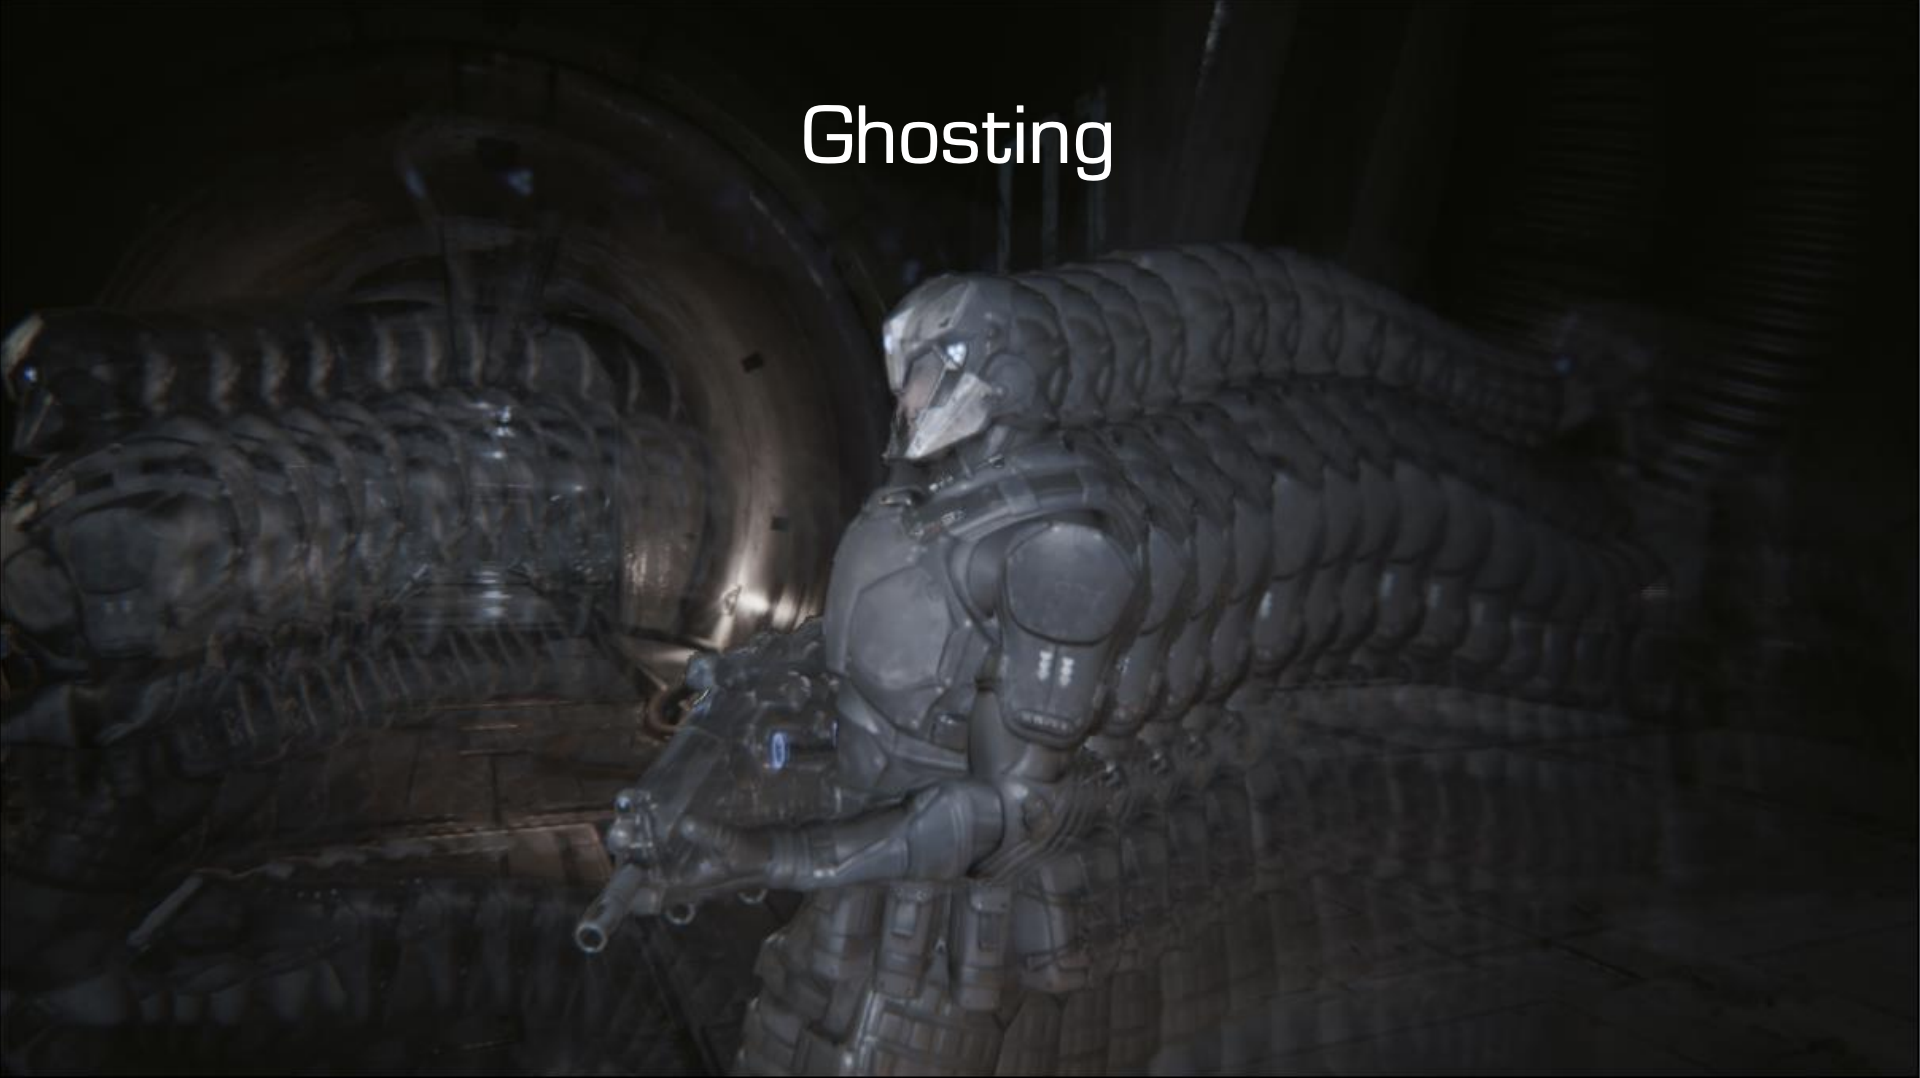
\includegraphics[width=.8\linewidth]{figures/ghosting.png}
    \caption{Ghosting\cite{unrealtaa}}
    \label{ghosting}
\end{figure}

\begin{minted}{glsl}
#version 330 core
out vec4 FragColor;

in vec2 TexCoords;

uniform sampler2D currentTexture;
uniform sampler2D historyAATexture;
uniform sampler2D motionTexture;


#define KERNEL_SIZE 9
const float step_w = 1.0 / 1920;
const float step_h = 1.0 / 1080;
const vec2 offset[KERNEL_SIZE] = vec2[KERNEL_SIZE](
    vec2(-step_w, -step_h), vec2(0.0, -step_h), vec2(step_w, -step_h),
    vec2(-step_w, 0.0), vec2(0.0, 0.0), vec2(step_w, 0.0),
    vec2(-step_w, step_h), vec2(0.0, step_h), vec2(step_w, step_h)
);

void main() {
    vec2 historyVel = texture(motionTexture, TexCoords).xy;
    vec2 uvLast = TexCoords + historyVel;

    vec4 maxVal = vec4(0.0f, 0.0f, 0.0f, 0.0f);
    vec4 minVal = vec4(1.0f, 1.0f, 1.0f, 0.0f);

    for (int i = 0; i < KERNEL_SIZE; ++i) {
        vec4 tmp = texture2D(historyAATexture, uvLast.xy + offset[i]);
        maxVal = max(tmp, maxVal);
        minVal = min(tmp, minVal);
    }

    vec4 color = mix(texture(currentTexture, TexCoords),
                     clamp(texture(historyAATexture, uvLast),minVal, maxVal),
                     0.60f);

    FragColor = color;
}
\end{minted}

\section{Sharpening kernel}

Debido a la naturaleza del temporal anti-aliasing la imagen final puede resultar demasiado suave. Los bordes quizás resulten algo difusos. Este efecto puede no ser del agrado del usuario. Una posible solución es usar un kernel de sharpening que resalta los bordes de la geometría.

\[
    \begin{bmatrix}
        0 & -1 & 0 \\
        -1 & 5 & -1 \\
        0 & -1 & 0
    \end{bmatrix}
\]

\begin{minted}{glsl}
#version 330 core
out vec4 FragColor;
in vec2 TexCoords;
uniform sampler2D finalTexture;

#define KERNEL_SIZE 9
const float kernel[KERNEL_SIZE] = float[KERNEL_SIZE](
    0.0, -1.0 , 0.0 ,
    -1.0 , 5.0 , -1.0 ,
    0.0 , -1.0 , 0.0
);
const float step_w = 1.0 / 1920;
const float step_h = 1.0 / 1080;
const vec2 offset[KERNEL_SIZE] = vec2[KERNEL_SIZE](
    vec2(-step_w, -step_h), vec2(0.0, -step_h), vec2(step_w, -step_h),
    vec2(-step_w, 0.0), vec2(0.0, 0.0), vec2(step_w, 0.0),
    vec2(-step_w, step_h), vec2(0.0, step_h), vec2(step_w, step_h)
);

void main(void)
{
    int i = 0;
    vec4 sum = vec4(0.0);

    vec4 tmp = texture2D(finalTexture, TexCoords.xy + offset[0]);
    sum += tmp * kernel[0];
    tmp = texture2D(finalTexture, TexCoords.st + offset[1]);
    sum += tmp * kernel[1];
    tmp = texture2D(finalTexture, TexCoords.st + offset[2]);
    sum += tmp * kernel[2];
    tmp = texture2D(finalTexture, TexCoords.st + offset[3]);
    sum += tmp * kernel[3];
    tmp = texture2D(finalTexture, TexCoords.st + offset[4]);
    sum += tmp * kernel[4];
    tmp = texture2D(finalTexture, TexCoords.st + offset[5]);
    sum += tmp * kernel[5];
    tmp = texture2D(finalTexture, TexCoords.st + offset[6]);
    sum += tmp * kernel[6];
    tmp = texture2D(finalTexture, TexCoords.st + offset[7]);
    sum += tmp * kernel[7];
    tmp = texture2D(finalTexture, TexCoords.st + offset[8]);
    sum += tmp * kernel[8];

    sum = clamp(sum, 0.0, 1.0);

    FragColor = sum;
}
\end{minted}

\chapter{Resultados}

A continuación se encuentran algunos resultados de la implementación del anti-aliasing temporal.

La figura~\ref{aaoff} contiene la imagen que creaba el motor sin modificaciones. Se puede ver una cantidad considerable de aliasing en el borde del cubo, al estar ligeramente inclinado. Activando el anti-aliasing temporal, como en las figuras~\ref{taa8} y~\ref{taa16}, se aprecia una mejora notable en la calidad de los bordes. Activando más samples la calidad aumenta.

El anti-aliasing temporal también mejora el aliasing en reflejos. Comparando las figura~\ref{shadowtaaOFF} con la figura~\ref{shadowtaaON} se puede apreciar un borde más suave, también en el interior de la geometría. Esto no es posible solucionarlo con un multisampling anti-aliasing tradicional.

Por último, en la figura~\ref{sharpOnsmall} se puede ver el efecto visual producido por el filtro de sharpening. Comparado con la figura~\ref{sharpOFFsmall} las bordes resaltan mucho más, y eliminan la suavidad de los bordes. Comparado con la imagen original (figura~\ref{sharpTAAOFFsmall}) puede resultar excesivo. Afortunadamente el filtro es opcional y el usuario final tiene la opción de activarlo o no, dependiendo de su preferencia.

\begin{figure}[!htbp]
    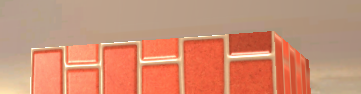
\includegraphics[width=.8\linewidth]{figures/taaoff.png}
    \caption{Anti-aliasing desactivado}
    \label{aaoff}
\end{figure}

\begin{figure}[!htbp]
    
\includegraphics[width=.8\linewidth]{figures/taa8.png}
    \caption{Temporal anti-aliasing con 8 samples}
    \label{taa8}
\end{figure}

\begin{figure}[!htbp]
    
\includegraphics[width=.8\linewidth]{figures/taa16.png}
    \caption{Temporal anti-aliasing con 16 samples}
    \label{taa16}
\end{figure}

\begin{figure}[!htbp]
    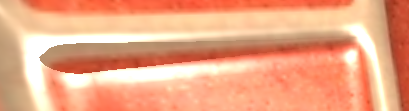
\includegraphics[width=.8\linewidth]{figures/shadowtaaOFF.png}
    \caption{Reflejos especulares con anti-aliasing apagado}
    \label{shadowtaaOFF}
\end{figure}

\begin{figure}[!htbp]
    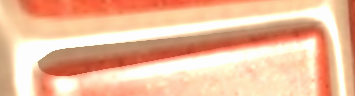
\includegraphics[width=.8\linewidth]{figures/shadowtaaON.png}
    \caption{Reflejos especulares con temporal anti-aliasing}
    \label{shadowtaaON}
\end{figure}

\begin{figure}[!htbp]
    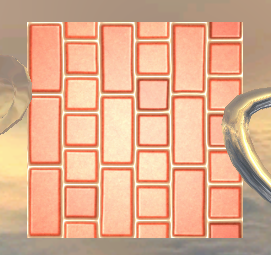
\includegraphics[width=.8\linewidth]{figures/sharpOFFsmall.png}
    \caption{Filtro de sharpening desactivado}
    \label{sharpOFFsmall}
\end{figure}

\begin{figure}[!htbp]
    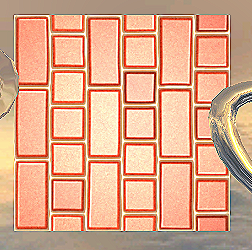
\includegraphics[width=.8\linewidth]{figures/sharpONsmall.png}
    \caption{Filtro de sharpening activado}
    \label{sharpOnsmall}
\end{figure}

\begin{figure}[!htbp]
    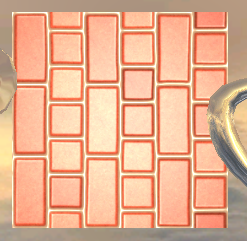
\includegraphics[width=.8\linewidth]{figures/sharpTAAOFFsmall.png}
    \caption{Temporal anti-aliasing desactivado}
    \label{sharpTAAOFFsmall}
\end{figure}

\chapter{Conclusión}

Para lograr unos resultados excelentes con respecto a la calidad de imagen es indispensable implementar un sistema de anti-aliasing robusto, capaz de solucionar los varios aspectos del aliasing. El approach que ha habido durante los últimos años refleja esta realidad fielmente. De pasar a usar multisampling y acelerarlo por hardware, a usar sistemas de post-procesado implementados completamente en software, pasando por métodos híbridos, hasta culminar en el anti-aliasing temporal.

El anti-aliasing temporal soluciona una gran parte de problemas del aliasing, como en bordes de geometría, en texturas, en reflejos especulares y además se puede reutilizar parte del pipeline (los motion vectors) para la implementación de un motion blur que solventa el aliasing de movimiento. Ademas de reaprovechar el pipeline para solventar el motion aliasing se puede usar para otros efectos visuales como el \GLS{SSAO}, que aportan todavía más realismo a las escenas. Su compatibilidad y rendimiento, al igual que los sistemas de post-procesado, hacen que sea un candidato perfecto para sistemas que se ejecutan en tiempo real, como los videojuegos.

Sin embargo, su implementación no es nada trivial. Si bien es cierto que su implementación para una imagen estática no requiere demasiada precisión, para escenas dinámicas, con reflejos y transparencias requieren que la implementación sea extremadamente precisa. Si no es así, aparecerán defectos visuales mucho peores que el aliasing, como por ejemplo el ghosting o un resultado excesivamente suave. Además no llegará a ser una solución drop-in, como pueden ser el FXAA o el SMAA, por ejemplo. Esos algoritmos, puramente de post-procesado, los puede llegar a inyectar el usuario, aunque el desarrollador no los haya incluido en su software. En cambio, el temporal anti-aliasing requiere información y modificaciones que están muy ligadas al motor gráfico usado.

Con la popularización del hardware especifico para tareas de aprendizaje automático, tanto en tarjetas gráficas como en dispositivos móviles, el siguiente paso en el campo del anti-aliasing puede llegar a ser un algoritmo de este tipo. Estos algoritmos aplicados al software en tiempo real todavía están en su infancia, pero en otros entornos se usan con muy buenos resultados.

En definitiva, el anti-aliasing temporal saca todo el potencial que ofrecen los motores gráficos y se convertirá en el sistema usado por defecto, reemplazando técnicas como el multisampling.

A un nivel más personal, este proyecto ha satisfecho una inquietud mía de sobre el funcionamiento de estas técnicas que tengo desde hace años. En un futuro se pretende extender el sistema para incluir mejoras como soporte para escenas dinámicas, transparencias, reflejos, motion blur, \Gls{SSAO}, etc.

% Bibliography:
\nocite{*}
\printbibliography{}

\listoffigures

% Index
\printthesisindex{}

\end{document}
